\documentclass[11pt,dvipdfmx]{jreport}
\usepackage{wuse_thesis}
\usepackage{indentfirst}
\usepackage{url}	% \url{}コマンド用.URLを表示する際に便利
\usepackage{graphicx}  % ←graphicx.styを用いてEPSを取り込む場合有効にする
\usepackage{listings,jvlisting} %日本語のコメントアウトをする場合jvlisting(もしくはjlisting)が必要

\usepackage{multirow}
\usepackage{array}

\usepackage{color}

\renewcommand{\lstlistingname}{Program}
\newcommand{\todo}[1]{\colorbox{yellow}{{\bf TODO}:}{\color{red} {\textbf{[#1]}}}}
			% 他のパッケージ・スタイルを使う場合には適宜追加

%ここからソースコードの表示に関する設定
\definecolor{darkgray}{rgb}{.4,.4,.4}
\definecolor{purple}{rgb}{0.65, 0.12, 0.82}

\lstdefinelanguage{JavaScript}{
  keywords={typeof, new, true, false, catch, function, return, null, catch, switch, var, if, in, while, do, else, case, break},
  keywordstyle=\color{blue}\bfseries,
  ndkeywords={class, export, boolean, throw, implements, import, this},
  ndkeywordstyle=\color{darkgray}\bfseries,
  identifierstyle=\color{black},
  sensitive=false,
  comment=[l]{//},
  morecomment=[s]{/*}{*/},
  commentstyle=\color{purple}\ttfamily,
  stringstyle={\small\ttfamily},
  morestring=[b]',
  morestring=[b]"
}

\lstset{
  basicstyle={\ttfamily},
  identifierstyle={\small},
  commentstyle={\smallitshape},
  keywordstyle={\small\bfseries},
  ndkeywordstyle={\small},
  stringstyle={\small\ttfamily},
  frame={tb},
  breaklines=true,
  columns=[l]{fullflexible},
  numbers=left,
  xrightmargin=0zw,
  xleftmargin=3zw,
  numberstyle={\scriptsize},
  stepnumber=1,
  numbersep=1zw,
  lineskip=-0.5ex
}
%ここまでソースコードの表示に関する設定

%%%%%%%%%%%%%%%%%%%%%%%%%%%%%%%%%%%%%%%%%%%%%%%%%%%%%%%%%%%%%%%%%%%%%%%%

%%%%%%%%%%%%%%%%%%%%%%%%%%%%%%%%%%%%%%%%%%%%%%%%%%%%%%%%%%%%%%%%%%%%%%%%

%%
%% 主に表紙を作成するための情報
%%

%%  タイトル(修論の場合は英語表記も指定)
\title{JavaScriptライブラリのテストコード変更内容に\\基づく後方互換性損失の検出}
%\etitle{Test\\Test\\Test}

%%  著者名(修論の場合は英語表記も指定)
\author{前川 大樹}
%\eauthor{Akinori Ihara}

%% 卒業論文・修士論文(以下のどちらかを選択)
\bachelar	% 卒業論文(4年生用)
%\master  	% 修士論文(M2用)

%%  学科・クラスタ
\department{システム工}
%\department{デザイン情報}
%\department{デザイン科学}

%%  学生番号
\studentid{60256245}

%%  卒業年度
\gyear{2023}		% 提出年が2022年なら,2021年度

%%  論文提出日
\date{2024年2月13日}	% 修士の場合は月(2021年2月)までとし,英語表記も指定
%\edate{February 2021}	% 修士の場合,こちら(英語表記)も有効化

%%%%%%%%%%%%%%%%%%%%%%%%%%%%%%%%%%%%%%%%%%%%%%%%%%%%%%%%%%%%%%%%%%%%%%%%

\begin{document}

\maketitle

%%
%%  概要
%%
\begin{abstract}
本研究では,ソフトウェアの後方互換性の損失をテストコードの変更内容に基づいて判定する手法を提案する.

ソフトウェア開発では,ライブラリと呼ばれる再利用可能なプログラムの利用により,開発者自身が同じ機能を再実装する必要がなくなり開発効率が向上する.ライブラリの機能追加や不具合修正のため,ライブラリに対して行われる変更は軽微な修正であっても破壊的変更が含まれることがある.破壊的変更を含むライブラリ更新をライブラリを利用するクライアントソフトウェアが適用すると,クライアントソフトウェアが実行時エラーになってしまうことがある.このような,更新後のライブラリがクライアントに影響を与えることを後方互換性を損失するという.ライブラリ開発者はクライアントに影響を与えないよう,ライブラリの後方互換性の損失有無をクライアントに正確に伝えることが求められる.

従来研究では,ライブラリの動作を検証するテストコードの変更有無に着目した後方互換性の損失の検出手法を提案している.しかし,テストコードはテストケースの実行手順の変更など,ライブラリの変更とは無関係に変更されることがあり,従来手法ではテストコードの変更内容は考慮されておらず誤検出が多い.本研究では,テストコード変更には後方互換性の損失に伴う変更と伴わない変更があると考え,テストコード変更内容を詳細に分析することで,後方互換性の損失をより正確に検出することを目指す.具体的には,後方互換性が損失するライブラリバージョンにおけるテストコードの変更内容を明らかにし,自動検出するツールを開発して後方互換性の損失の検出精度を検証する.


\end{abstract}

%%  目次
\tableofcontents

%%  図目次 (図目次をいれたければ以下のコメントをはずす)
%\listoffigures

%%  表目次 (表目次をいれたければ以下のコメントをはずす)
%\listoftables

\newpage
\pagenumbering{arabic}	% 以降のページ番号を算用数字に

%%%%%%%%%%%%%%%%%%%%%%%%%%%%%%%%%%%%%%%%%%%%%%%%%%%%%%%%%%%%%%%%%%%%%%%%

%%
%%  本文はここから
%%

\chapter{はじめに}
ソフトウェア開発では,ライブラリと呼ばれる再利用可能なプログラムの利用により,開発者自身が同じ機能を再実装する必要がなくなり開発効率が向上する\cite{shared-software}\cite{effect-on-developer}.ソフトウェアは新機能の追加,バグ修正などによって頻繁に更新されており,ライブラリも例外ではない\cite{library-analysis}.ライブラリの更新には,脆弱性の修正などライブラリを利用するクライアントソフトウェア(以降,クライアント)にとって重要な変更が含まれることがあり,これによりクライアントは依存ライブラリの更新を余儀なくされることも多い.クライアント開発者が依存ライブラリを更新する際,更新後ライブラリに機能削除や仕様変更といったクライアントに影響を与える変更が含まれる場合,更新前の仕様を前提とするクライアントと,更新後ライブラリのソースコードに不整合が生じ,クライアントが実行時エラーになってしまうことがある.このような,更新後のライブラリがクライアントに影響を与えることを後方互換性を損失するという.ライブラリ開発者はクライアントに影響を与えないよう,ライブラリの後方互換性の損失有無をクライアントに正確に伝えることが求められる.

ライブラリ開発者が更新後ライブラリの後方互換性の有無をクライアントに伝える手法として,セマンティックバージョニング\footnote{\url{https://semver.org}}がある.セマンティックバージョニングは,ライブラリ開発者がライブラリにバージョン名を付与するための規則で,バージョン名を「1.0.0」などの3つの数字で表す.それぞれの数字は,「メジャー.マイナー.パッチ」と呼ばれ,後方互換性を損失する変更ではメジャー,後方互換性を維持する変更ではマイナー,またはパッチの値を増やし新しいバージョン名を付与する.しかし,バージョン名の付与はライブラリ開発者が手動で行うため,後方互換性を損失しているにも関わらず誤ってマイナーやパッチに分類されてしまうことがある.Javaのような静的型付け言語では,バージョニングシステムを使用しなくても型情報が後方互換性の損失を判断することに役立つ\cite{java-api-diff-tool}.例えば,ライブラリのメソッドの型が変更された場合,当該メソッドを利用するクライアントコードはコンパイルできなくなる.一方JavaScriptなどの動的型付け言語では,型情報やコンパイルがないため,誤ったバージョン名による影響はクライアントの実行時まで検出されないことが多い.この課題に対して,JavaScriptライブラリの後方互換性の損失を検出する研究が行われている.

松田らは,後方互換性を損失するライブラリの更新は,プログラムの更新と合わせてテストコードも修正すると考え,テストコードの変更有無による後方互換性損失の検出手法を提案した\cite{matsuda}.しかし,テストコードの変更内容を考慮しておらず,テストコードの実行手順の修正のようなライブラリの更新とは無関係のテストコード変更についても後方互換性を損失したと誤検出する.誤検出により後方互換性の損失を過剰に検出してしまうと,ライブラリの利用者は必要以上に慎重になり,ライブラリの新機能の活用や脆弱性修正の適用が遅れる可能性がある.逆に,後方互換性の損失を見落とすと,ライブラリを利用するソフトウェアの実行時エラーなどの問題が生じる.したがって,後方互換性の損失を正確に検出することは,ソフトウェアの品質維持と開発効率の向上に直結する.本研究では,テストコード変更には後方互換性の損失に伴う変更と伴わない変更があると考え,テストコードの変更内容を詳細に分析することで,後方互換性の損失をより正確に検出することを目指す.具体的には,2つのResearch Question(RQ)に回答する.

\begin{itemize}
  \item RQ1:後方互換性の損失に伴うテストコード変更とは何か?
  \item RQ2:テストコード変更内容に基づく後方互換性損失の検出手法の有効性はどの程度か?
\end{itemize}

RQ1では,ライブラリ更新が後方互換性の損失を含む際,それに伴ってテストコードをどのように変更するかを分析し,後方互換性の損失を検出する手がかりとなるテストコード変更内容を明らかにする.RQ2では,これらの変更内容を自動検出するツールを開発し,後方互換性損失の検出精度を検証する.

以降,本論文では,\ref{chap:backward-compatibility}章で後方互換性の損失がクライアントに与える影響と関連研究,本研究の位置付けを述べ,\ref{chap:rq1}章,\ref{chap:rq2}章では,設定したRQにおけるそれぞれの分析手法,結果,考察を述べる.続く\ref{chap:heuristic}章では,妥当性の脅威を述べ,最後に\ref{chap:end}章で本論文をまとめる.

\chapter{後方互換性の損失}\label{chap:backward-compatibility}

\section{後方互換性の損失の原因}
ライブラリが後方互換性を損失する原因として,ライブラリが提供するAPI(アプリケーションプログラミングインターフェース)の振る舞いの変更がある.メソッド,シグネチャ,例外,入出力データ形式など,APIの振る舞いの変更は全てクライアントに影響を与える可能性がある.APIの機能拡張やバグ修正であっても,拡張された機能が存在しないことや,壊れている動作に依存していた場合,クライアントにエラーを引き起こす原因になる.一方,提供するAPIの追加や,ライブラリの内部でのみ使用されるモジュールの変更では一般的にクライアントが影響を受けることはない.Java言語では,privateアクセス修飾子等を利用することで,クライアントに影響を与えることなく,ライブラリの内部でのみ利用するモジュールを変更することができる.しかし,JavaScript言語ではライブラリのどのモジュールをAPIとしてクライアントに提供し,どのモジュールを内部で使用するかを明確に定義していることが少ない.ライブラリ開発者が内部だけの使用を意図してモジュールの振る舞いを変更していたとしても,多数のクライアントが当該モジュールを使用しており変更の影響を受けることもある.例として,ユーザインターフェースを構築するライブラリReactの15.3.2から15.4.0へのマイナーアップデート\footnote{\url{https://github.com/facebook/react/compare/v15.3.2...v15.4.0}}では,react/lib/ReactMountモジュールを刷新する変更が行われた.ライブラリ開発者は,内部使用のみを意図していたが,多数のクライアントが当該モジュールを使用しており,変更の影響を受けた\footnote{\url{https://github.com/rekit/rekit/issues/16}}.

\section{クライアントに与える影響}
JavaScriptライブラリの後方互換性の損失がクライアントに与える影響を調査した研究\cite{impact-analysis-for-clients}では,npm\footnote{\url{https://www.npmjs.com/}}から384件のクライアントを調査し,11.7%が後方互換性の損失による影響を受けたことを示している.また,後方互換性を損失した全64件のリリースのうち,約44%がマイナーリリースとパッチリリースであったことも示されており,ライブラリ開発者にとってバージョン名を適切に付与することは難しいとわかる.ライブラリのバージョン名に誤った値が付与されている場合,クライアント開発者が後方互換性を維持することを期待してライブラリバージョンを適用し,エラーが引き起こされてしまうことになる.例として,2016年12月,デバッグ用のAPIを提供するライブラリdebugの2.3.3から2.4.0へのマイナーアップデート\footnote{\url{https://github.com/debug-js/debug/compare/2.3.3...2.4.0}}では,ソースコード中に単純なスペルミスによるバグが混入し\footnote{\url{https://github.com/debug-js/debug/issues/347}},新バージョンを適用したクライアントはエラーを引き起こした.バグは1時間以内に修正されたが\footnote{\url{https://github.com/debug-js/debug/pull/356}},debugは12月だけでも2,700万回以上ダウンロードされ,多数のクライアントが影響を受けた.

\section{関連研究}
ライブラリ開発者が誤ったバージョン名を付与し,クライアントにエラーを引き起こすことを防ぐため,後方互換性の損失を検出する研究が行われている.

Fooらは,Java,Python,Ruby言語を対象に,ライブラリバージョン間のメソッドの差分を解析することによる後方互換性の有無の判定手法を提案した\cite{foo}.しかし,この手法はメソッドに行われた変更は全て後方互換性を損失したと検出するため,リファクタリングなど外部から見た振る舞いに変化がない変更であっても後方互換性を損失したと誤検出する.また,コールグラフ作成の困難さから,動的型付け言語であるRubyやPythonの後方互換性の有無はほとんど判断できていない.

Møllerらは,クライアント開発者がクライアントの動作を検証するために作成したテスト(以降,クライアントテスト)を利用し,動的型付け言語であるJavaScriptの型情報をクライアントテストによって補うことで後方互換性の損失の検出を試みた\cite{type-regression-testing}\cite{model-based-testing}.しかし,この手法ではクライアントテストを実行するためにかなりの時間がかかることがある.本研究では,クライアントテストといったライブラリ外の資源は利用せず,ライブラリに付属するテストを静的解析することで後方互換性の損失を検出する手法を提案する.

Kraaijeveldは,後方互換性を損失する変更を,ライブラリが定義している関数名やパラメータ数の変更と定義し,後方互換性の損失の検出を試みた\cite{detecting-breaking-changes-in-js-apis}.ただし,この手法では関数やクラスの入出力形式の変更や,例外処理の追加などによる後方互換性の損失を検出することができない.本研究では,ライブラリの動作を検証するテストコードを利用する.テストコードは,テスト対象となる関数やクラスの入出力の情報や例外の情報を有しており,ライブラリの後方互換性の損失の種類を絞ることなく検出することを目指す.



\section{先行研究}
関連研究が示すとおり,動的型付け言語であるJavaScript言語における後方互換性の損失の検出は多くの場合に困難である.

松田らは,JavaScriptライブラリに付属するテストコードが,テスト対象となる関数やクラスの入出力の情報を含んでおり,型情報を補うことができる点に着目し,ライブラリのテストコード変更有無に基づく後方互換性の検出手法を提案した\cite{matsuda}(以降,従来手法).ライブラリを更新する際,その動作を検証するテストコードも通常更新する.したがって,テストコードの変更有無から後方互換性の損失を検出できると示唆される.従来手法は,テストコードをテストケースの追加,変更,削除,変更なしに分類し,テストケースを変更・削除したバージョンのソフトウェアは後方互換性を損失したと検出する.ただし,APIの仕様変更に伴って,新しい仕様の動作を保証するためにテストケースを追加することや,テストの実行手順の修正や可読性向上のためのフォーマッティングなど,プログラムの変更とは無関係にテストコードを変更することも考えられ,そのような変更は誤検出の原因になる.

\section{キーアイデア}\label{sec:key-idea}

\begin{figure}[t]
  \centering
  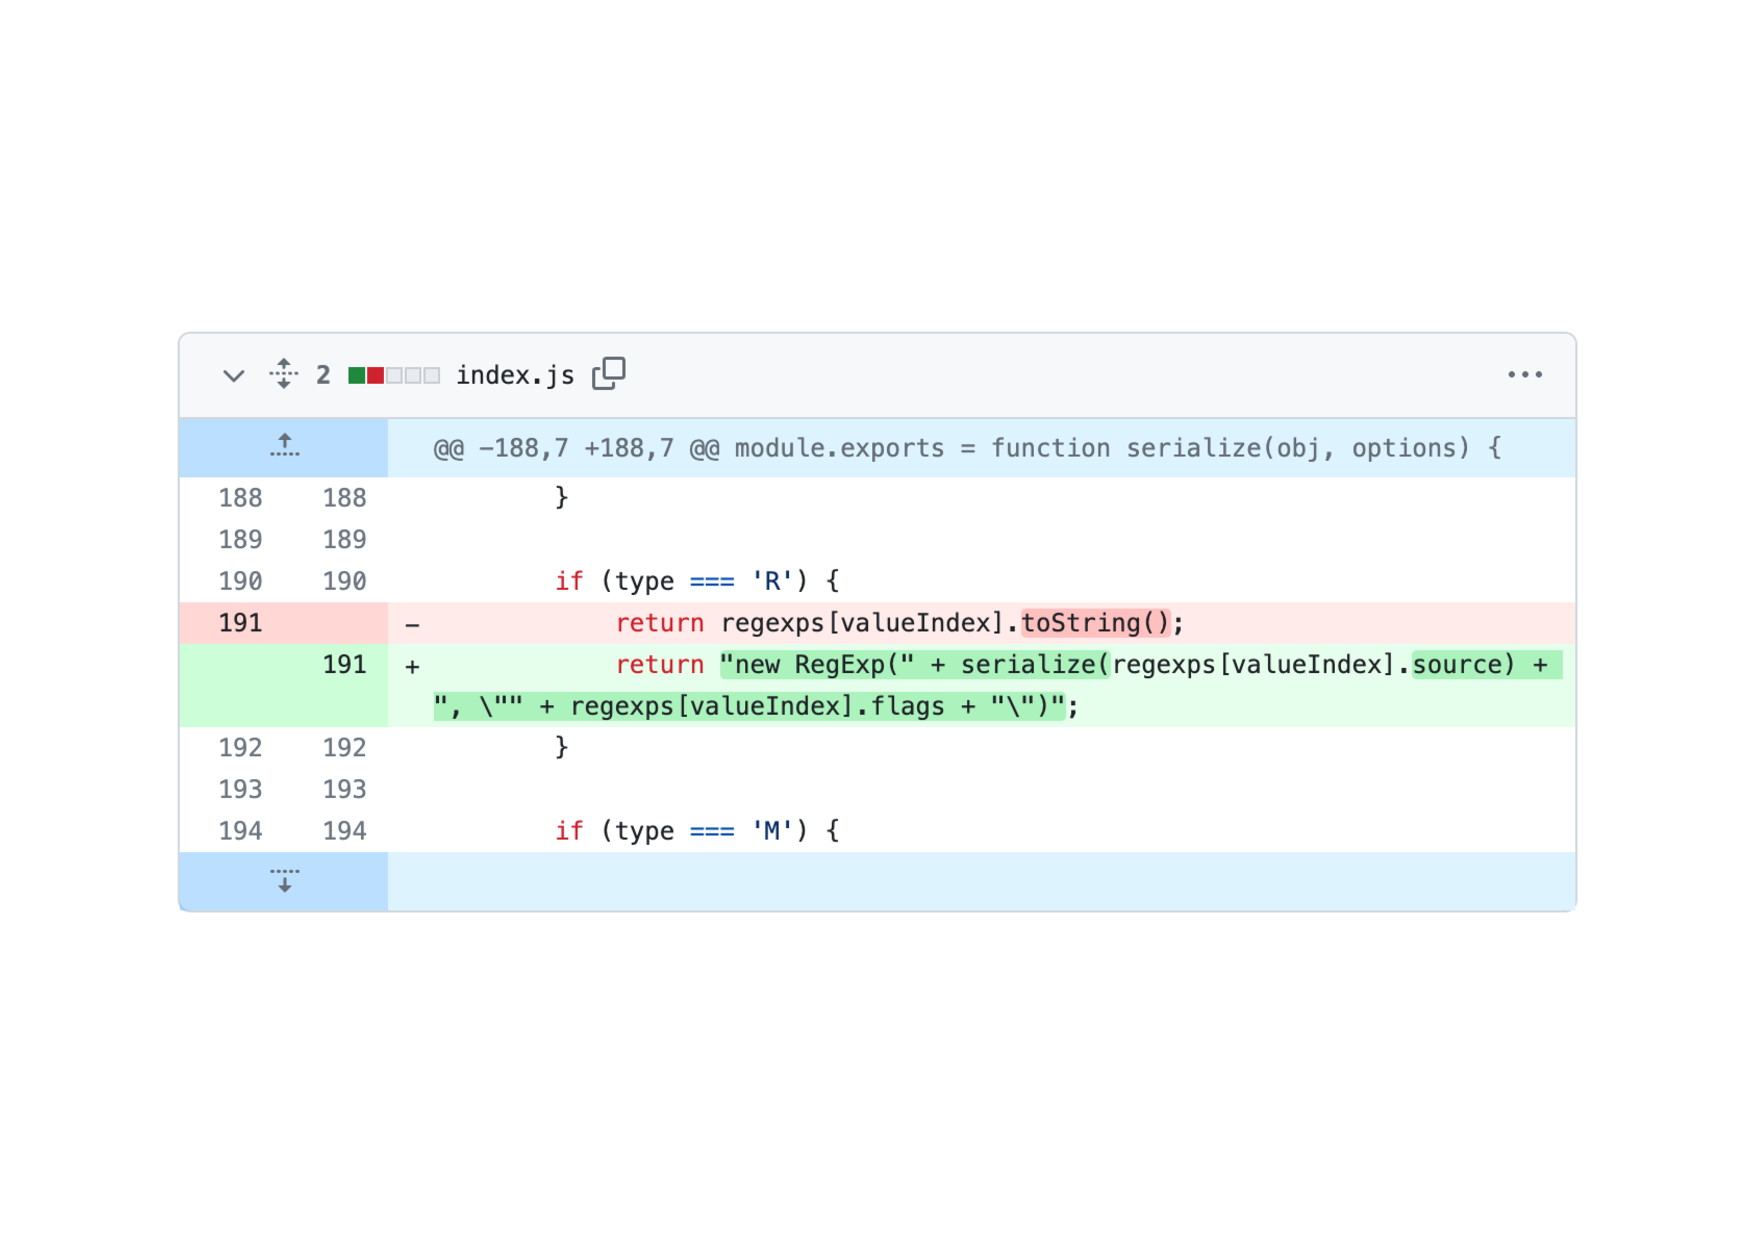
\includegraphics[width=1.0\linewidth]{fig/rq1/serialize-javascript/index.pdf}
  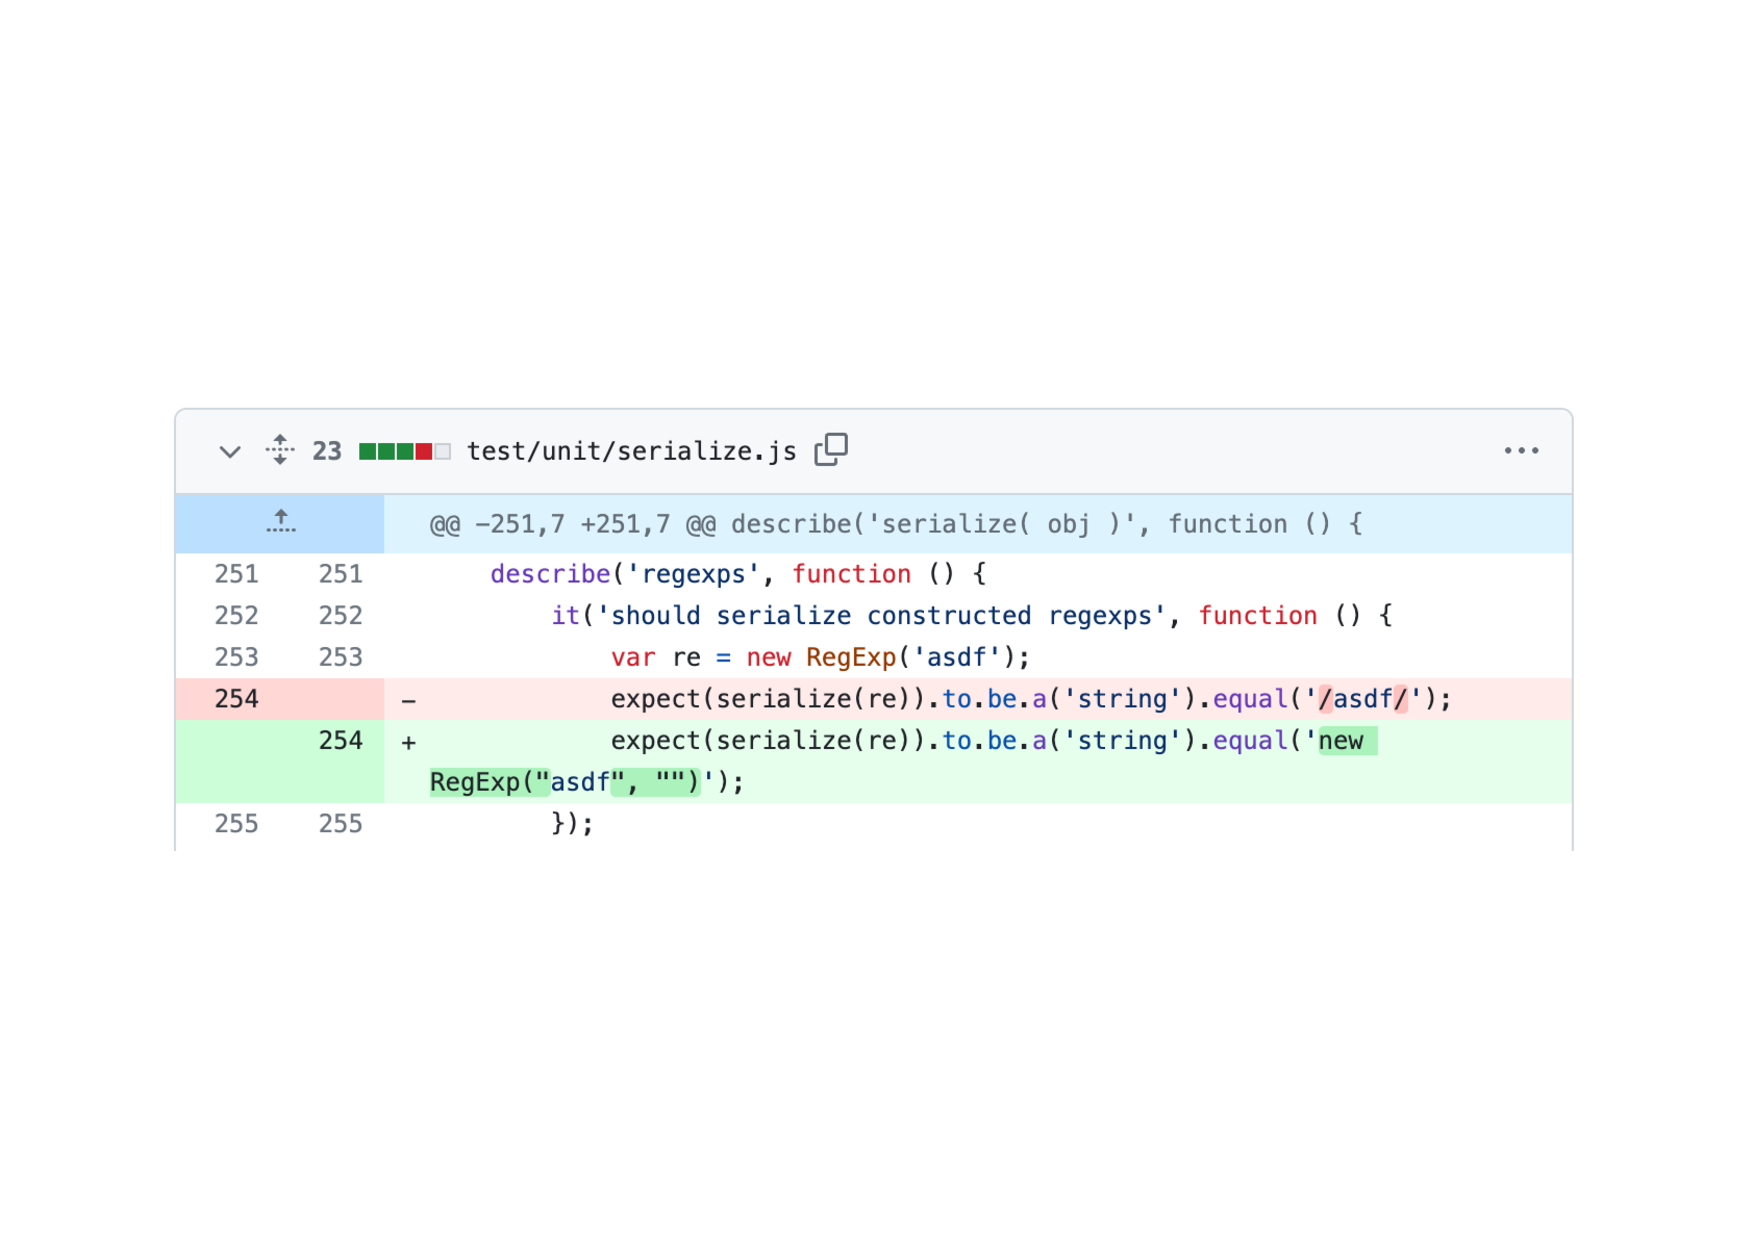
\includegraphics[width=1.0\linewidth]{fig/rq1/serialize-javascript/index.test.pdf}
  \caption{serialize-javascriptのバージョン2.1.0から2.1.1への変更}
  \label{fig:motivation}
\end{figure}

従来手法では,テストコードの変更を4つに分類することで後方互換性損失の検出を試みたが誤検出が多い結果となった.本研究では,テストコード変更には後方互換性の損失に伴う変更と伴わない変更があると考え,テストコード変更内容に基づく後方互換性の損失の検出手法を提案し精度を検証する.

図\ref{fig:motivation}は,後方互換性の損失に伴うテストコード変更の例として,JavaScriptオブジェクトを文字列に変換する関数を提供するライブラリserialize-javascriptのバージョン2.1.0から2.1.1へのパッチアップデート\footnote{\url{https://github.com/yahoo/serialize-javascript/compare/v2.1.0...v2.1.1}}を示す.上部がソースコード,下部がテストコードのそれぞれの変更内容である.ソースコードの191行目で,190行目の条件に合致する特定の入力に対する関数の返り値が変更されている.この変更に伴って,対応するテストコードも修正されている.テストコードの254行目の変更では,テスト対象となる関数とパラメータはそのままで,期待する返り値のみ変更されている.後方互換性の損失に伴わないテストコード変更は,テストコードの実行手順の修正や,可読性向上のためのフォーマッティングなどが考えられる.このように,テストコードの変更内容には後方互換性の損失に伴う変更と伴わない変更があるため,テストコードの変更内容をより詳細に分析することで,後方互換性の損失を正確に検出することを目指す.続く\ref{chap:rq1}章では,後方互換性の損失を含むライブラリ更新に伴うテストコードの変更内容を分析し,\ref{chap:rq2}章で後方互換性の損失に伴うテストコードの変更内容を自動検出するツールを開発し後方互換性の損失の検出精度を従来手法と比較検証する.

\chapter{RQ1:後方互換性の損失に伴うテストコード変更とは何か?}\label{chap:rq1}

\section{概要}
本章では,後方互換性の損失を含むライブラリ更新に伴うテストコードの変更内容を分析し,後方互換性の損失を検出する手掛かりとなるテストコードの変更内容を明らかにする.具体的には,各ライブラリバージョンに対して,後方互換性の有無とテストコードの変更内容を目視で調査する.

\section{分析手法}

\subsection{後方互換性の有無の判定}\label{subsec:kouhougokanseinohantei}
後方互換性の有無の判定には,従来手法と同様,Mujahidらの手法を使用する.Mujahidらは,ライブラリの後方互換性の損失をクライアントテストを実行することで検出する手法を提案した\cite{mujahid}.後方互換性を損失する変更を加えられたライブラリバージョンでは,その影響を受けるクライアントテストの結果が更新前後で成功から失敗に変化することを手法の根拠としている.本分析も同様に,対象ライブラリのクライアントに対し,次の手順で後方互換性の有無を判定する.

\begin{enumerate}
  \item クライアントテストを実行する.テストが失敗した場合は分析対象外とする.
  \item ライブラリのバージョンを新しいものに更新し,クライアントテストを実行する.クライアントテストが失敗した場合,後方互換性を損失したと判定する.
\end{enumerate}

\subsection{テストコード変更内容の目視分類}
テストコード変更内容を目視分類するために,テストコードの構成要素をまとめる.本研究では,プログラムのテストの中でも単体テストを対象とする.単体テストとは,関数やクラスなどのプログラムを構成する単位(ユニット)が開発者の期待通りに動作するかを検証するテスト手法である.単体テストを実施する際は,テスト対象ユニットに対応するテストスイートを用意する必要がある.テストスイートとは,テストの目的や条件が似ているテストケースの集合を指す.テストケースは,テスト項目の最小単位であり,テスト対象への入力と期待される結果(期待値)の組み合わせで構成する.入力値と期待値を受け取ってプログラムが正しく動作しているか検証する仕組みをアサーションと呼ぶ.

\begin{lstlisting}[caption=Calculator.js, label=Calculator.js]
class Calculator {
  add(a, b) {
    return a + b;
  }
}
\end{lstlisting}

\begin{lstlisting}[caption=Calculator.test.js, label=Calculator.test.js]
import { Calculator } from './Calculator';

describe('Calculator', () => {
  let calculator;

  beforeEach(() => {
    calculator = new Calculator();
  });

  test('should add two positive numbers', () => {
    if (calculator) {
      expect(calculator.add(1, 1)).toBe(2);
    }
  });
});
\end{lstlisting}


Program~\ref{Calculator.js},Program~\ref{Calculator.test.js}は,JavaScriptにおけるテストコードの例を示す.Program~\ref{Calculator.js}は,テスト対象となるクラス{\verb|Calculator|}が定義されている.このクラスに含まれるメソッド{\verb|add()|}は,2つの引数を受け取り足し合わせた値を返す.Program~\ref{Calculator.test.js}は,{\verb|Calculator|}クラスを単体テストによって検証するファイルで,JavaScript向けテストフレームワークJest\footnote{\url{https://jestjs.io/}}を使用して記述している.

Program~\ref{Calculator.test.js}は,3行目の{\verb|describe|}関数でテストスイートを宣言し,10行目の{\verb|test|}関数により1つのテストケースを定義している.テストスイートやテストケースは,何を検証するかが記述されるラベルと,動作を検証するテスト用関数を引数に取る.6行目から7行目の{\verb|beforeEach|}関数で,テストフィクスチャと呼ばれる,テストデータの初期化などのテストの事前条件を定義する.例では,{\verb|Calculator|}クラスをインスタンス化している.10行目から12行目で定義されるテストケースは,11行目で{\verb|if|}文によりテストの前提条件を記述し,12行目のアサーションで{\verb|Calculator.add()|}に対し1と1を入力したときの動作を検証している.この場合,期待する結果は2であるため,{\verb|toBe|}節で結果が2となる.以上より,本研究ではJavaScript言語のテストコードの構成要素として次の5件を定義する.

\begin{itemize}
  \setlength{\itemsep}{0cm}
  \item テストスイート
  \item テストケース
  \item アサーション(入力値,期待値を含む)
  \item 前提条件
  \item テストフィクスチャ
\end{itemize}

テストコードの変更内容として,テストコードの構成要素それぞれを追加,変更,削除する変更内容が考えられる.アサーションの期待値,入力値はテストコードの最小単位であるため変更のみ考慮し,前提条件については追加,削除も前提条件が変更されたと考えられるため変更のみを考慮する.テストスイート・テストケースのラベルの変更,テストフレームワークの変更,可読性向上のためのフォーマッティングなどテストコードの振る舞いに関わらない変更については,リファクタリングとする.以上を踏まえ,本研究ではテストコードの変更内容として次の11件を考慮する.

\begin{itemize}
  \setlength{\itemsep}{0cm}
  \item テストスイートの追加
  \item テストスイートの削除
  \item テストケースの追加
  \item テストケースの削除
  \item アサーションの追加
  \item アサーションの削除
  \item アサーションの入力値の変更
  \item アサーションの期待値の変更
  \item テストの前提条件の変更
  \item テストフィクスチャの変更
  \item リファクタリング
\end{itemize}



\section{データセット}\label{rq1:datasets}
データセットとして,従来研究\cite{matsuda}で収集されたライブラリバージョン群を使用する.従来研究では,ライブラリの人気度を示すnpmスコア~\footnote{\url{https://npms.io}}が上位500件以内で,各バージョンのコミットにおけるテスト実行時の成功率が100%であることを条件にnpm\footnote{\url{https://www.npmjs.com/}}から2,111件のライブラリバージョンを収集した.本調査では,このデータセットから,ライブラリテストに変更があるライブラリバージョン1,027件を抽出し,95%の信頼区間でサンプリングした280件を対象とする.分析対象とするライブラリと,各ライブラリのいずれかに依存するクライアントとの組み合わせは,Mujahidらのデータセットから抽出した.

\section{分析結果}\label{seq:rq1-result}

\begin{figure}[t]
  \centering
  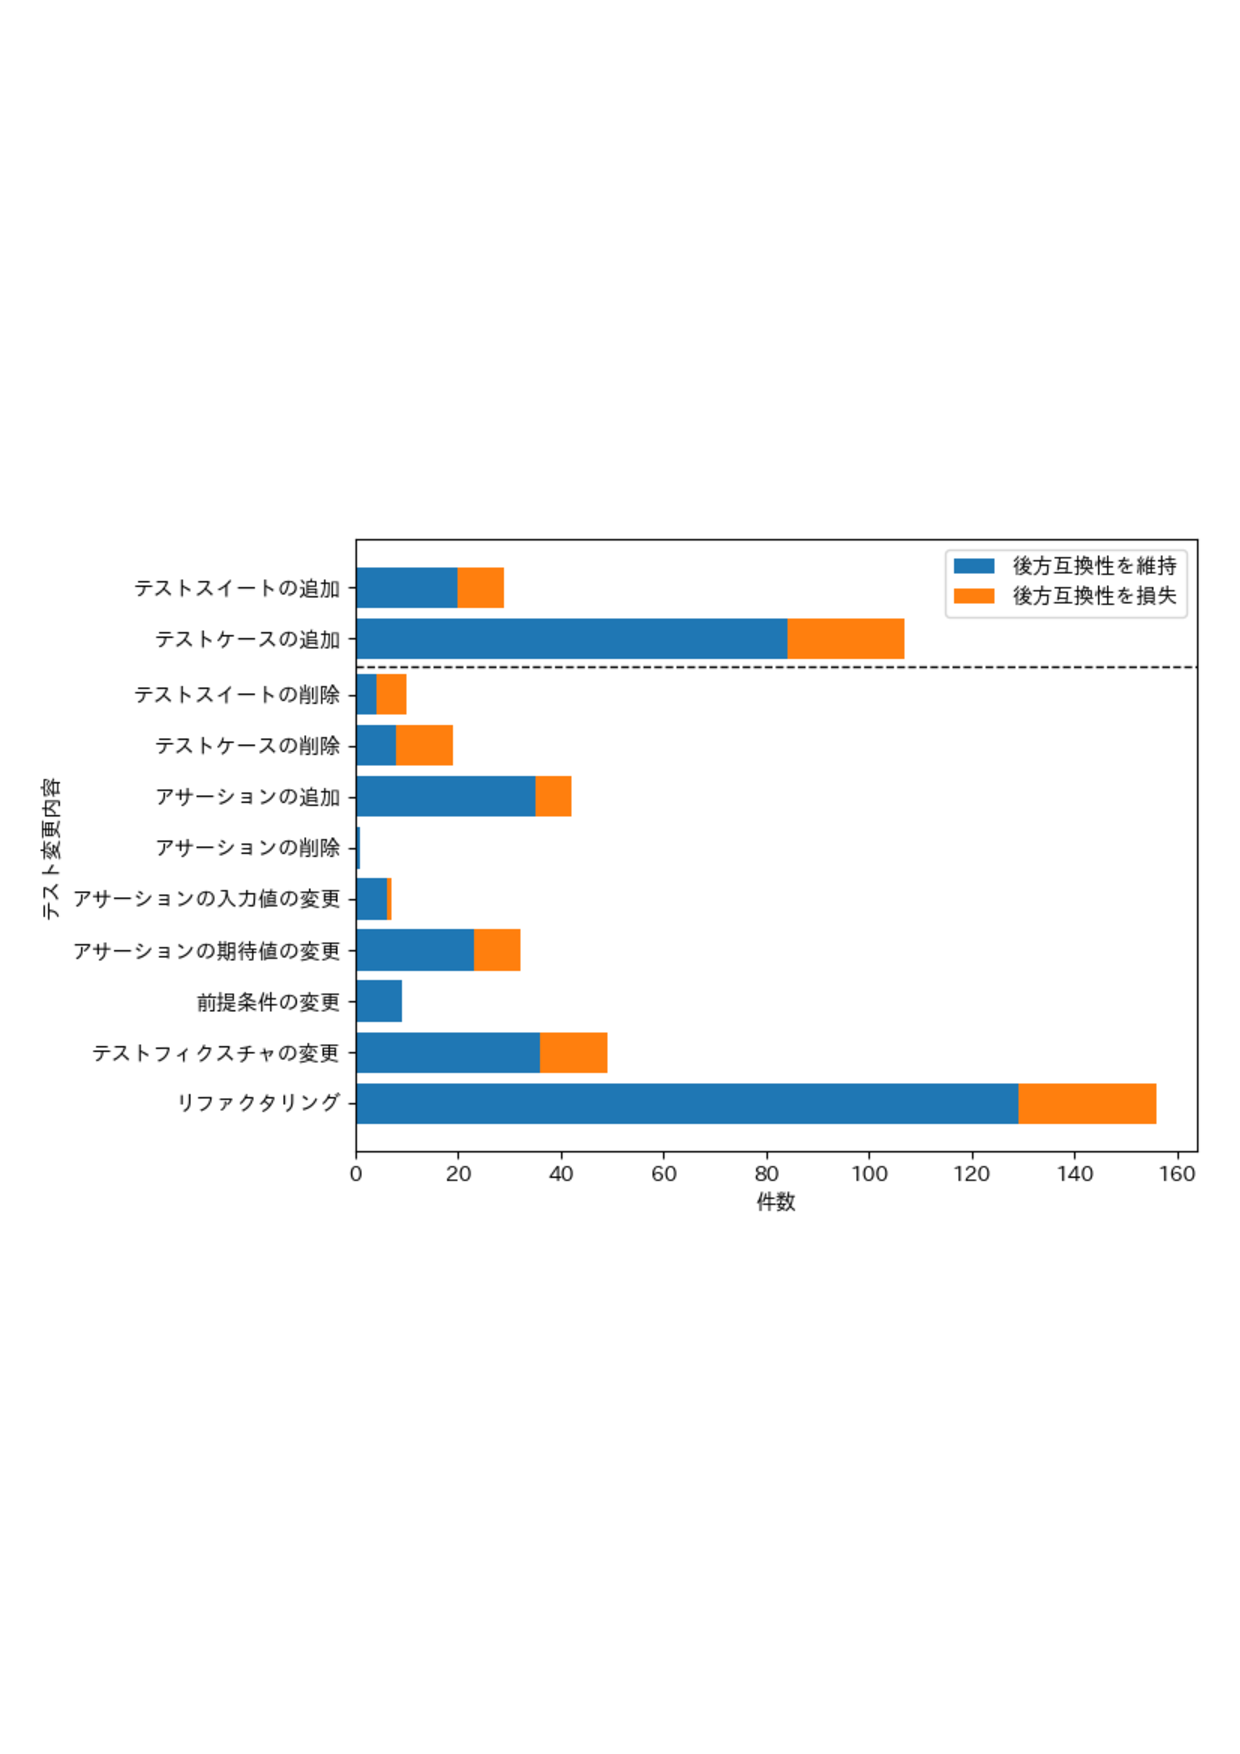
\includegraphics[width=1.0\linewidth]{fig/barh-test-pattern.pdf}
  \caption{テスト変更内容ごとの実際の後方互換性}
  \label{fig:test_pattern}
\end{figure}

図\ref{fig:test_pattern}は,テスト変更内容ごとの後方互換性の有無を横棒積み上げ棒グラフで示す.横軸は各テストコード変更の発生件数,縦軸は各テストコード変更内容である.破線より上は,従来手法で後方互換性を維持すると判定するテスト変更内容であり,破線より下は従来手法で後方互換性を損失すると判定するテスト変更内容である.

\subsection{従来手法で後方互換性を維持すると判定するテスト変更内容}
従来手法で後方互換性を維持すると判定するテスト変更内容は,テストスイートの追加,テストケースの追加である.これらは,後方互換性を維持するライブラリ更新に伴う場合が多いため,従来手法で誤検出となる主な原因ではない.ただし,後方互換性を損失するライブラリ更新に伴ってテストスイートやテストケースを追加する場合もある.具体的な例は\ref{subsec:add-test}項で述べる.

\subsection{従来手法で後方互換性を損失すると判定するテスト変更内容}
従来手法で後方互換性を損失すると判定するテスト変更内容は,テストスイートの削除,テストケースの削除,アサーションの追加,アサーションの削除,アサーションの入力値の変更,アサーションの期待値の変更,前提条件の変更,テストフィクスチャの変更,リファクタリングである.このうち,リファクタリングは後方互換性を維持するライブラリ更新に伴う場合が多く,件数も多いため従来手法で誤検出となる主な原因であるとわかる.一方,リファクタリングが後方互換性を損失するライブラリ更新に伴う場合もある.これは,後方互換性を損失するライブラリ更新に伴って,無関係にテストがリファクタリングされることがあることを示す.テストスイートの削除,テストケースの削除は,後方互換性を損失するライブラリ更新に伴う場合が多いため,従来手法で誤検出となる主な原因ではない.ただし,後方互換性を維持するライブラリ更新に伴ってテストスイートやテストケースを削除する場合もある.具体的な例は\ref{subsec:delete-test}項で述べる.アサーションの追加,アサーションの入力値の変更,アサーションの期待値の変更,前提条件の変更は,後方互換性を維持するライブラリ更新に伴う場合が多く,従来手法で誤検出となる主な原因である.ただし,後方互換性を損失するライブラリ更新に伴って,アサーションを追加したり,アサーションの入力値,アサーションの期待値を変更する場合もある.具体的な例は,それぞれ\ref{subsec:add-test}項,\ref{subsec:change-test}項で述べる.テストフィクスチャの変更は,テストデータの初期化や事前条件を定義する性質上,変更時のテストコードの影響範囲が広く,後方互換性の損失との関係を分析することが困難であるため,本研究では対象としない.

続く\ref{rq2:kousatu}節では,テスト変更内容をテストコード追加,テストコード削除,テストコード変更に分けて,後方互換性を損失するライブラリ更新に伴うテストコード変更内容,伴わないテストコード変更内容をそれぞれ例を挙げて考察し,後方互換性の損失を検出する手掛かりとなるテストコード変更内容を特定する.

\section{考察}\label{sec:rq1.kousatu}

\subsection{テストコード追加}\label{subsec:add-test}

\begin{figure}[t]
  \centering
  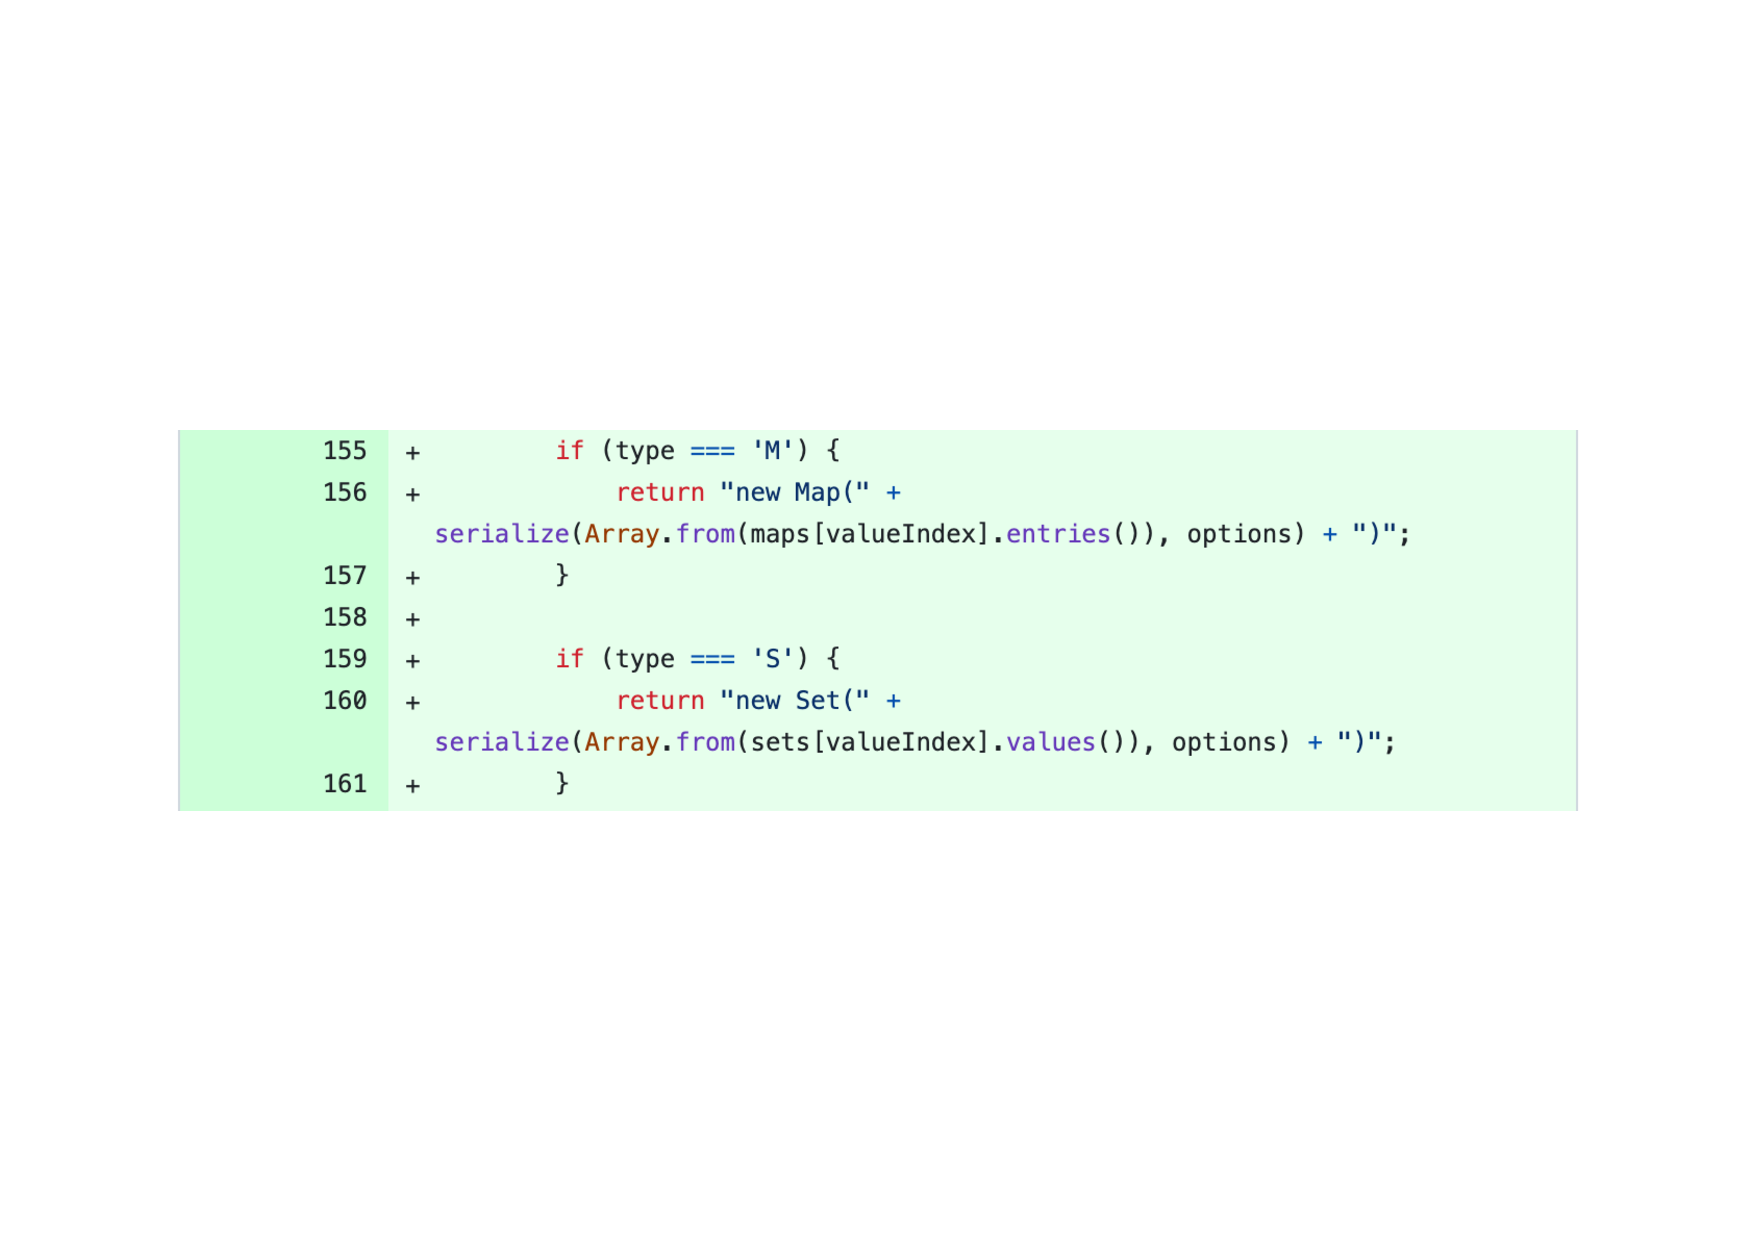
\includegraphics[width=1.0\linewidth]{fig/rq1/set-map/map.pdf}
  \caption{serialize-javascriptのバージョン1.6.1から1.7.0のソースコード変更差分}
  \label{fig:rq1.insert-test-src}
\end{figure}

\begin{figure}[t]
  \centering
  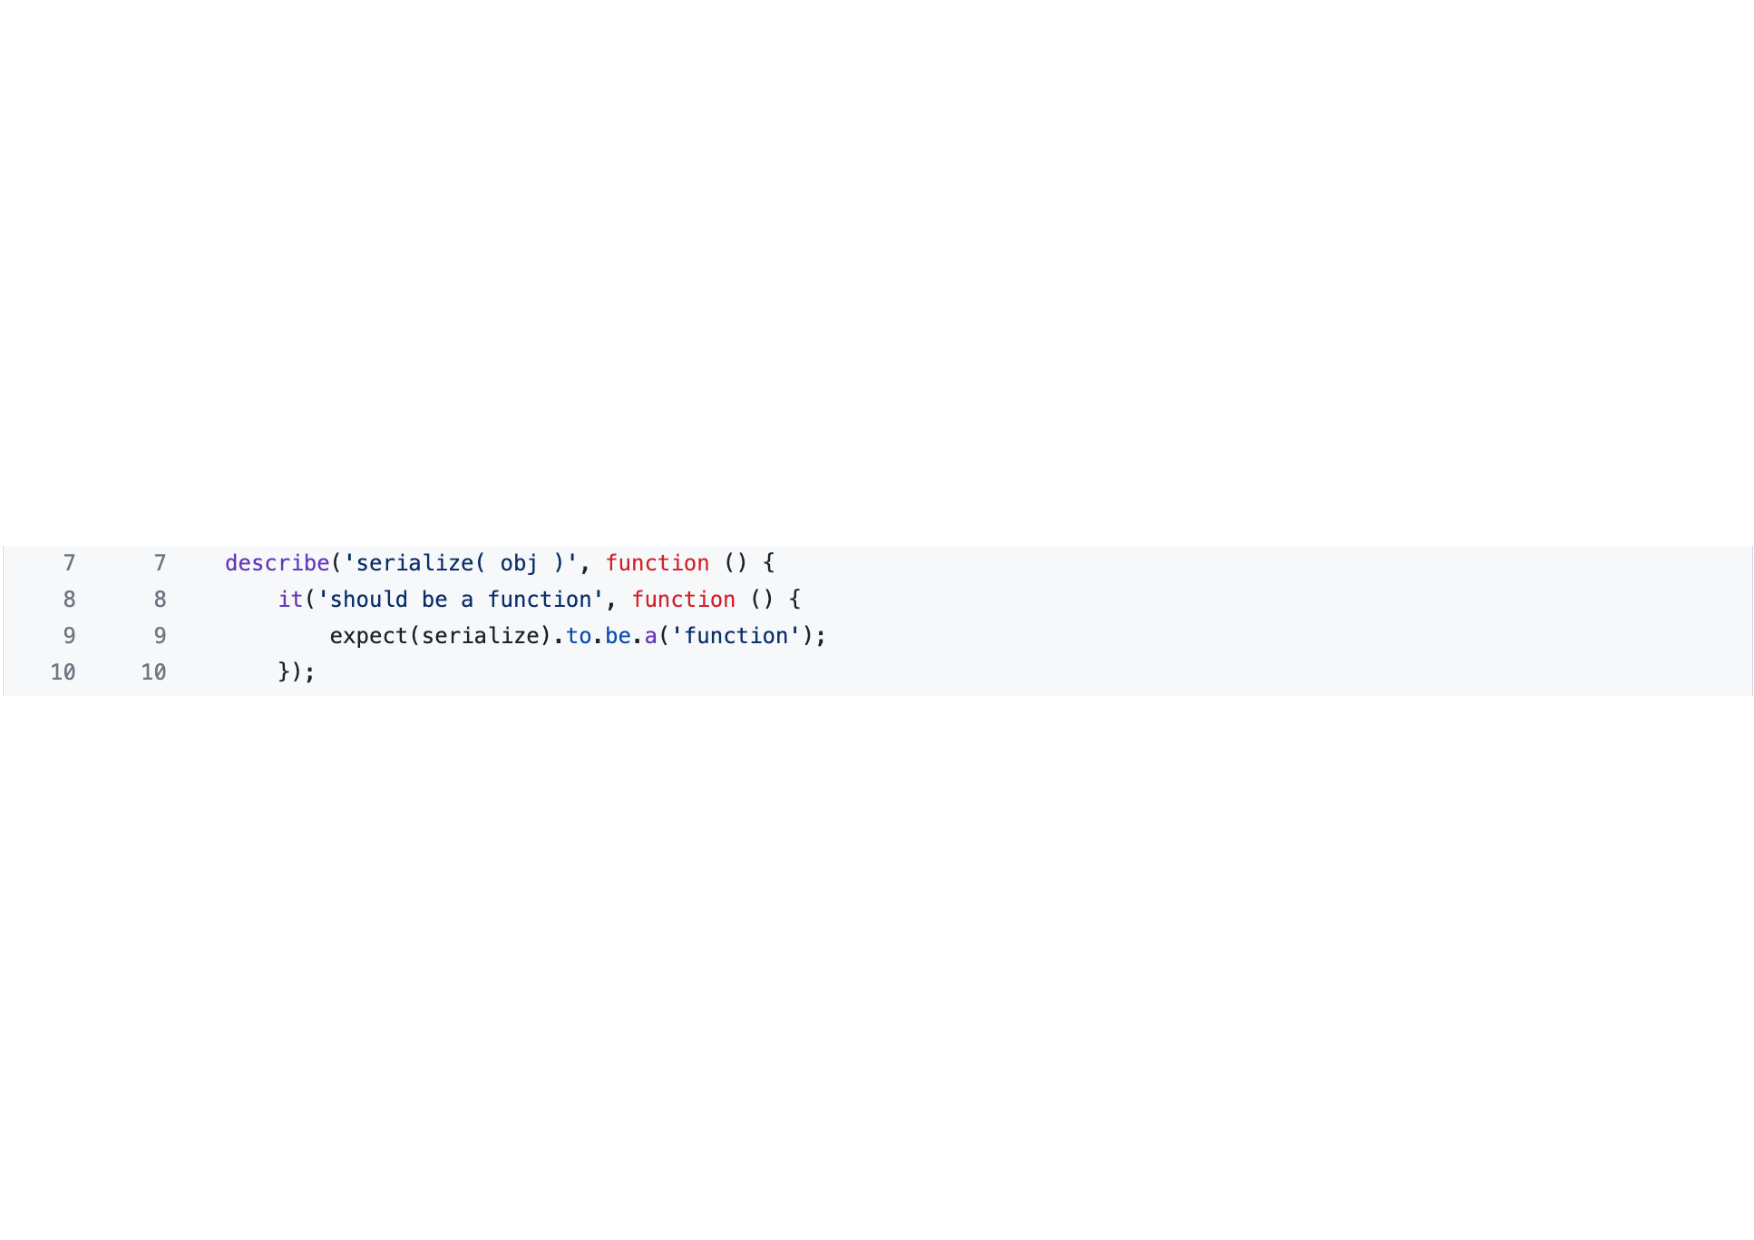
\includegraphics[width=1.0\linewidth]{fig/rq1/set-map/map.test.1.pdf}
  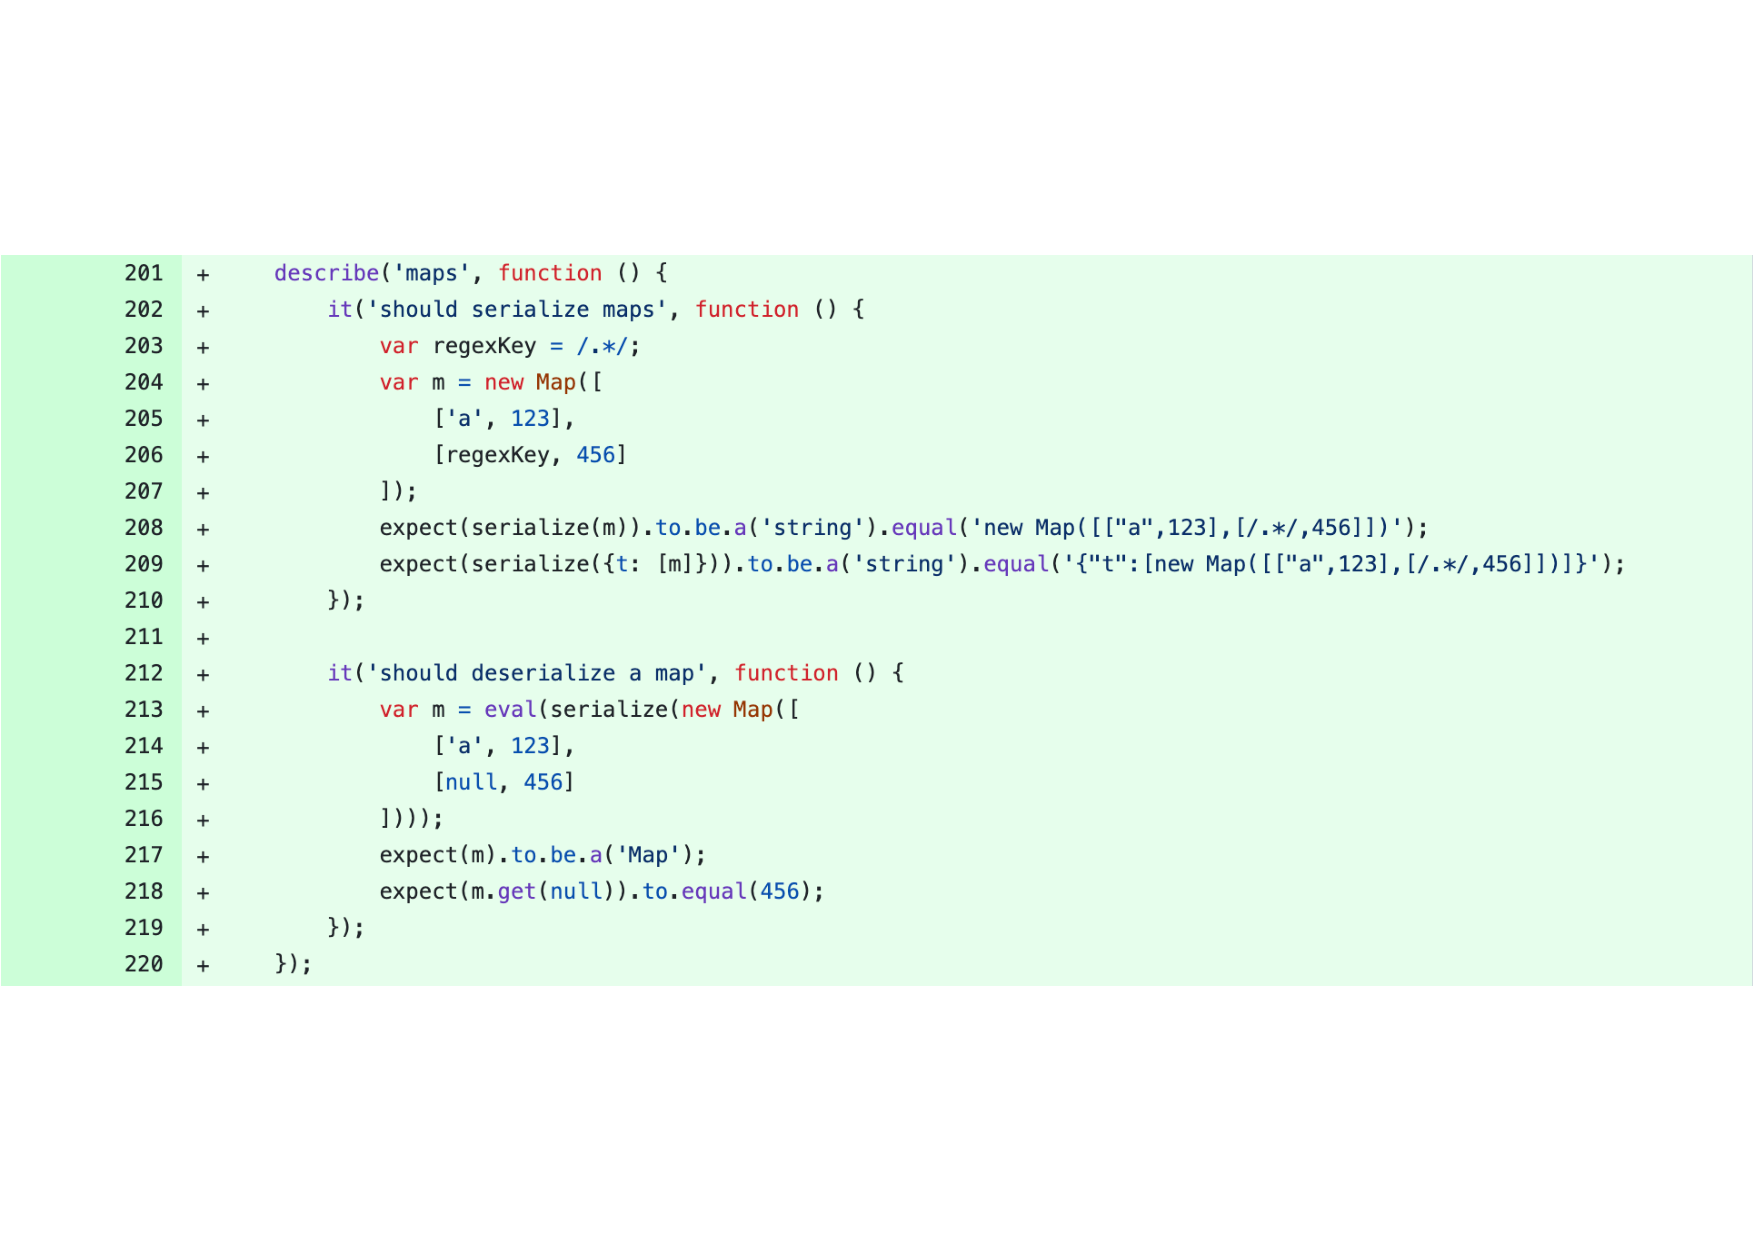
\includegraphics[width=1.0\linewidth]{fig/rq1/set-map/map.test.2.pdf}
  \caption{serialize-javascriptのバージョン1.6.1から1.7.0のテストコード変更差分}
  \label{fig:rq1.insert-test-test}
\end{figure}

テストコード追加は,テスト対象となるAPIの追加など後方互換性を維持するライブラリ更新に伴う場合が多い.ただし,後方互換性を損失するライブラリ更新に伴ってテストコードが追加されることがある.例として,JavaScriptオブジェクトを文字列に変換するAPIを提供するライブラリserialize-javascriptのバージョン1.6.1から1.7.0へのマイナーアップデート\footnote{\url{https://github.com/yahoo/serialize- javascript/compare/v1.6.1...v1.7.0}}を挙げる.図\ref{fig:rq1.insert-test-src}はソースコードの変更差分,図\ref{fig:rq1.insert-test-test}はテストコードの変更差分を示す.この変更では,関数{\verb|serialize|}に,JavaScriptの{\verb|Map|}型のデータを文字列に変換する機能が追加された(図\ref{fig:rq1.insert-test-src},155行目から157行目).この変更に伴って,関数{\verb|serialize|}に関するテストスイート(図\ref{fig:rq1.insert-test-test},7行目)に,新しく{\verb|Map|}型のデータが正確に文字列に変換されるかを検証するテストスイートが追加された(図\ref{fig:rq1.insert-test-test},201行目から220行目).バージョン1.6.1では,関数{\verb|serialize|}は{\verb|Map|}型の入力を文字列に変換する機能を持っていないため,文字列に変換されないことに依存しているクライアントはバージョン更新の際に返り値が新しくなったことによる影響を受ける.このようなAPIの機能拡張による後方互換性の損失は,図\ref{fig:rq1.insert-test-test}で示すように既存のテストスイート内にテストコードが追加されるという特徴があるため,既存のテストスイート内にテストスイート,テストケース,アサーションが追加された場合,ライブラリの後方互換性が損失したと判断できると考えられる.

\subsection{テストコード削除}\label{subsec:delete-test}

\begin{figure}[t]
  \centering
  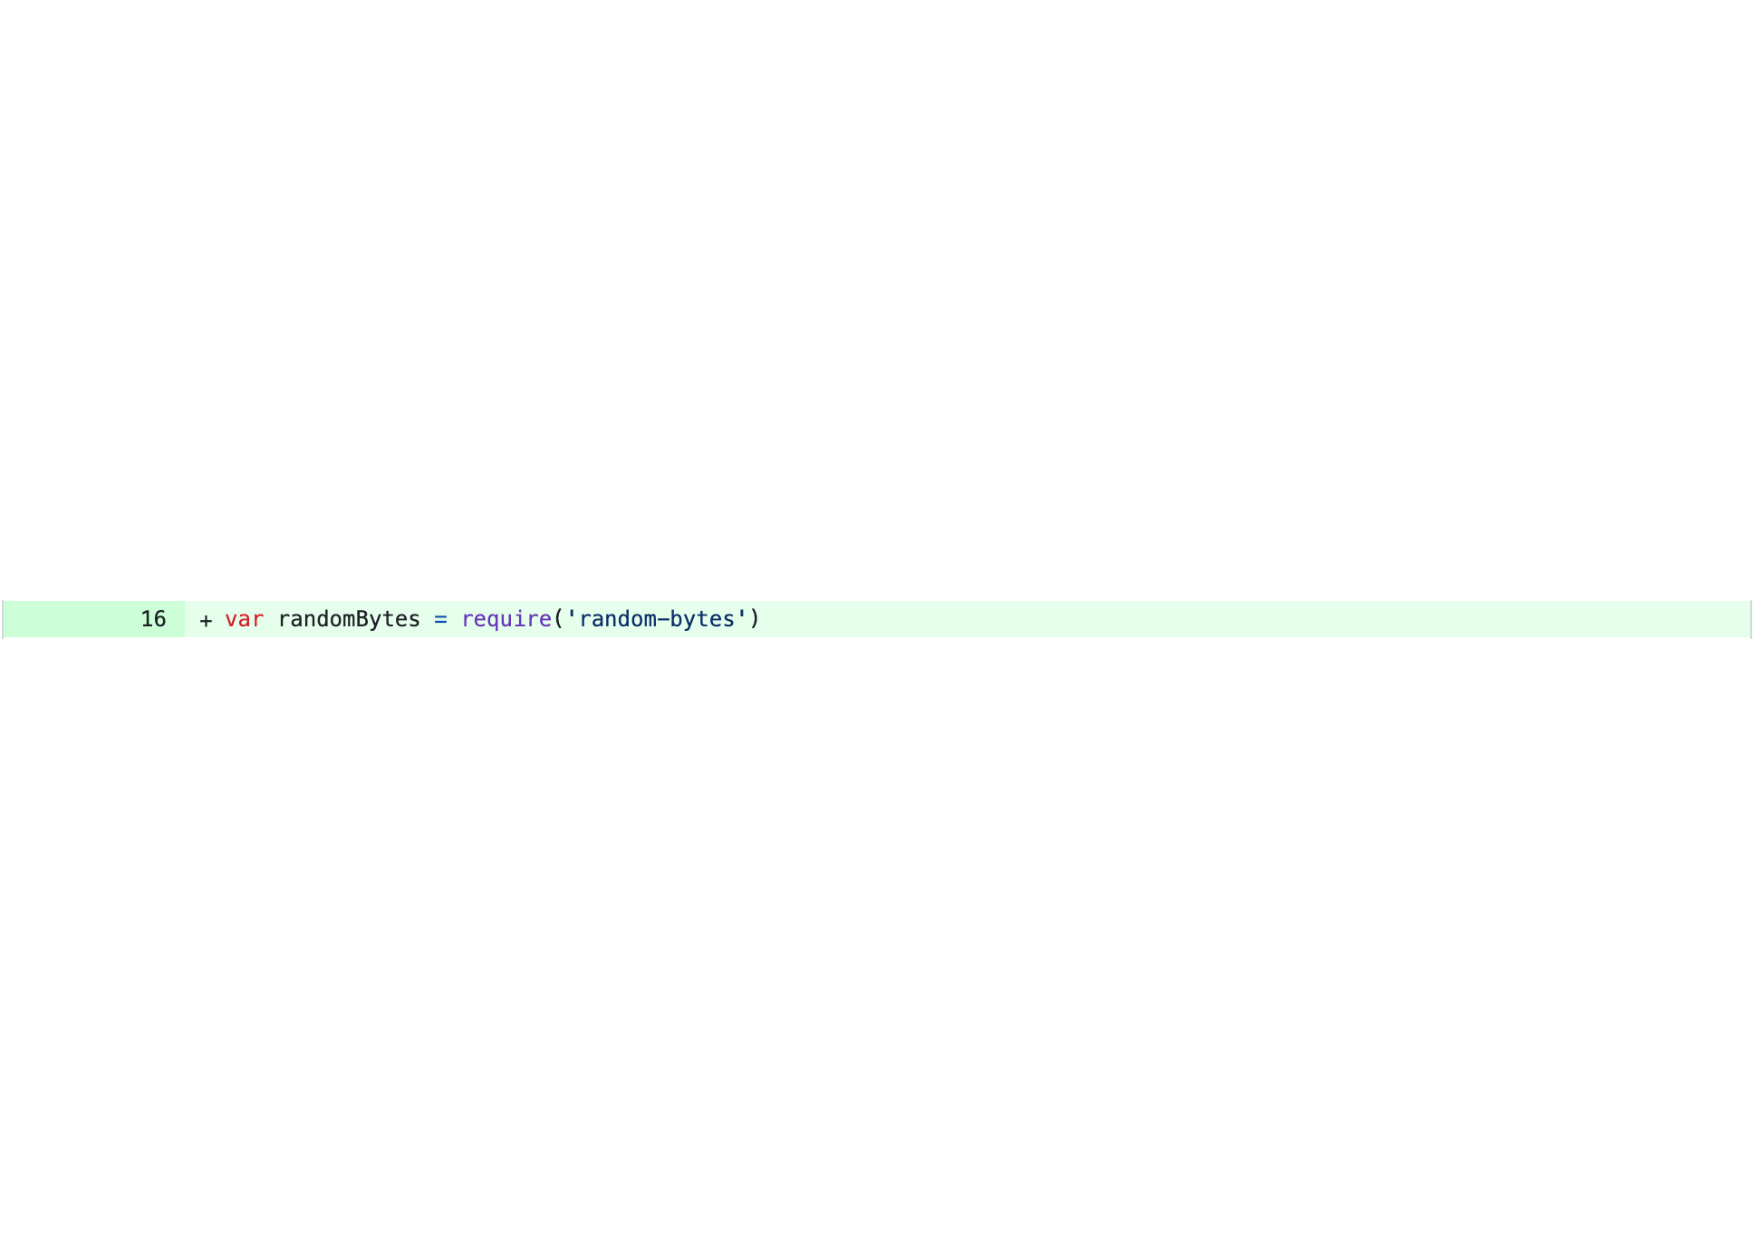
\includegraphics[width=1.0\linewidth]{fig/rq1/uuid/randomBytes2.pdf}
  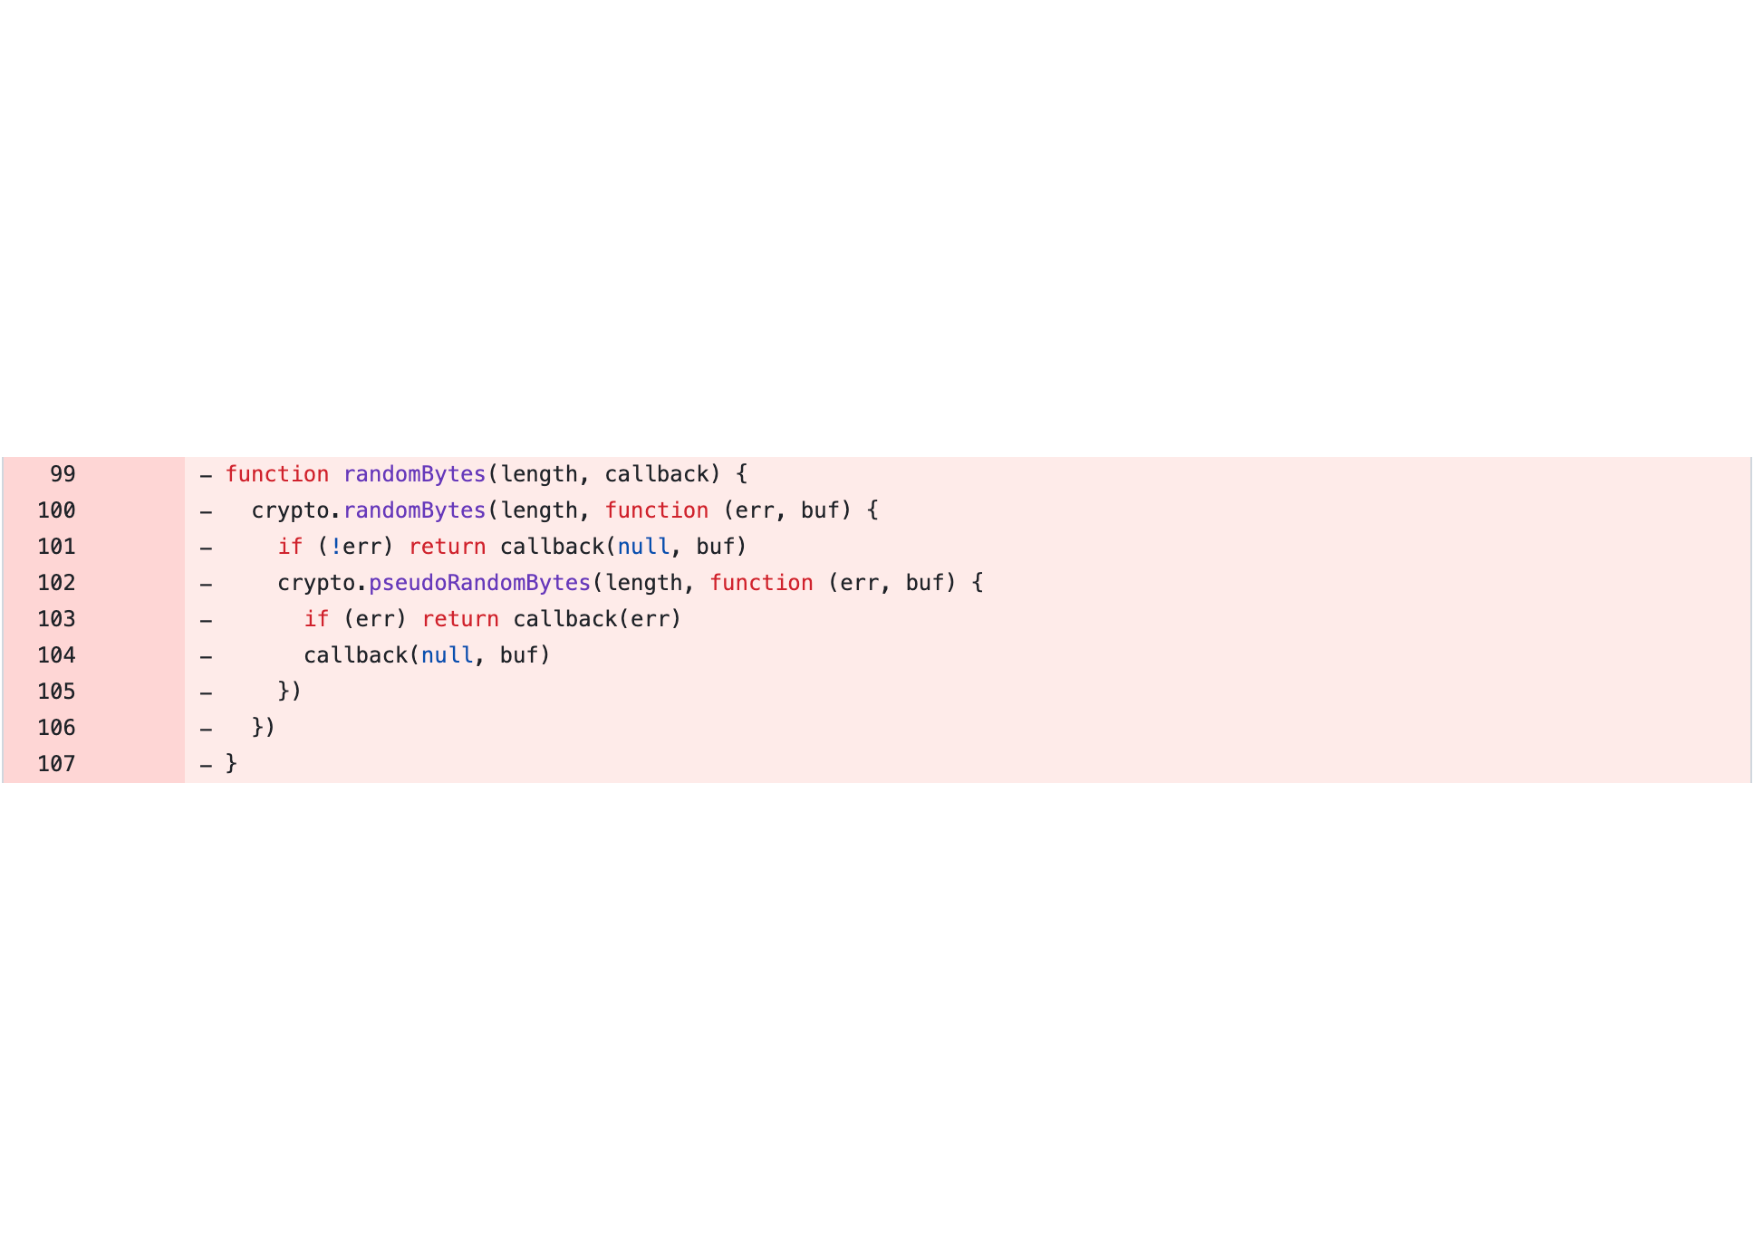
\includegraphics[width=1.0\linewidth]{fig/rq1/uuid/randomByte.pdf}
  \caption{uid-safeのバージョン2.0.0から2.1.0のソースコード変更差分}
  \label{fig:rq1.delete-test-src}
\end{figure}

\begin{figure}[t]
  \centering
  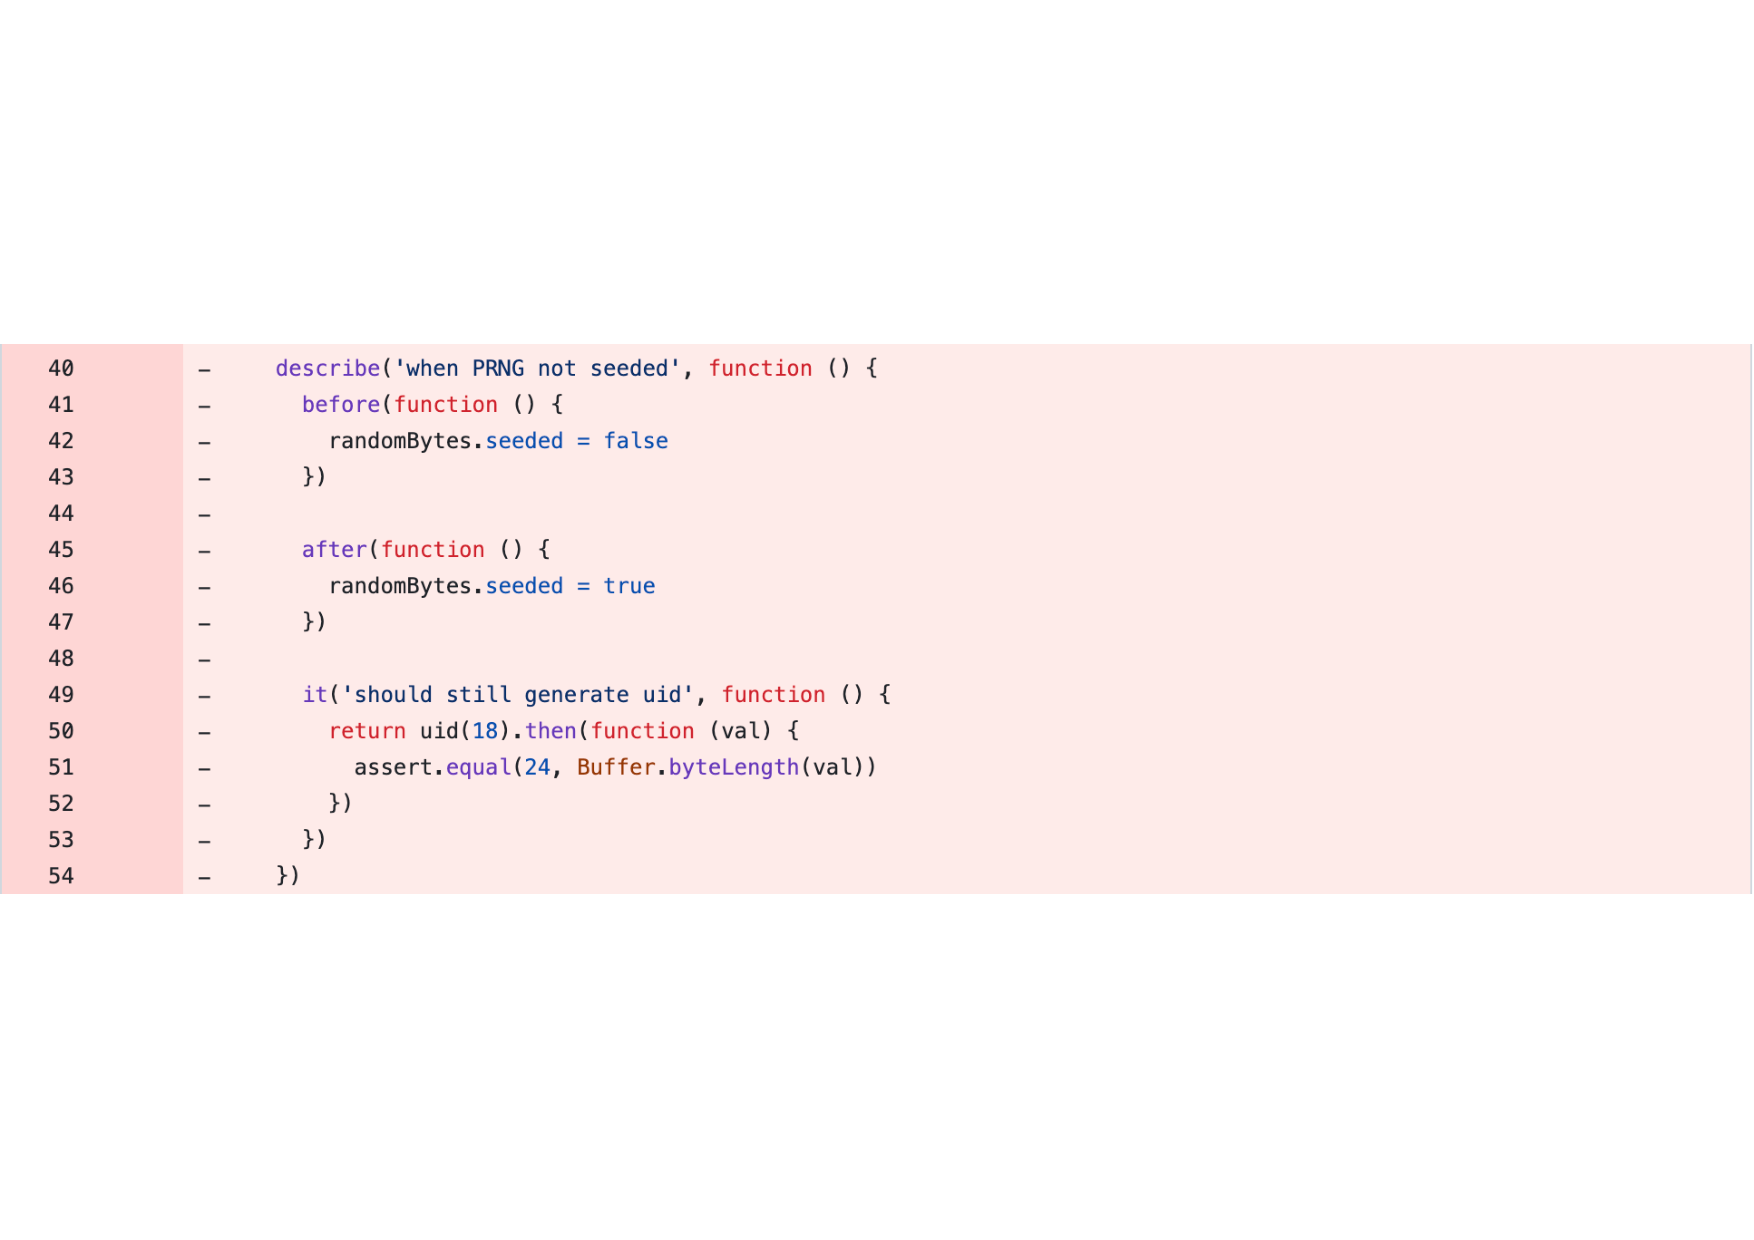
\includegraphics[width=1.0\linewidth]{fig/rq1/uuid/randomByte-test.pdf}
  \caption{uid-safeのバージョン2.0.0から2.1.0のテストコード変更差分}
  \label{fig:rq1.delete-test-test}
\end{figure}

テストコード削除は,テスト対象となるAPIの削除など後方互換性を損失するライブラリ更新に伴う場合が多い.ただし,後方互換性を維持するライブラリ更新に伴ってテストコードが削除されることがある.例として,暗号化されたUIDを生成するAPIを提供するライブラリuid-safeのバージョン2.0.0から2.1.0へのマイナーアップデート\footnote{\url{https://github.com/crypto-utils/uid-safe/compare/2.0.0...2.1.0}}を挙げる.図\ref{fig:rq1.delete-test-src}はソースコードの変更差分,図\ref{fig:rq1.delete-test-test}はテストコードの変更差分を示す.この変更では,セキュリティ上の問題から,ランダムなバイト列を生成する関数{\verb|randomBytes|}を削除(図\ref{fig:rq1.delete-test-src},99行目から107行目)し,同等のモジュールに置き換えている(図\ref{fig:rq1.delete-test-src},16行目).この変更に伴って,関数{\verb|randomBytes|}の動作を検証するテストスイートが削除されている(図\ref{fig:rq1.delete-test-test},40行目から54行目).モジュールの置き換え前後で関数{\verb|randomBytes|}の振る舞いが全く同じ場合,後方互換性が維持される.本研究では,\ref{subsec:kouhougokanseinohantei}章で述べた通り,後方互換性の有無の判定にクライアントテストを利用している.このようなモジュールに置き換える例では,振る舞いの変化が限定的になるため,クライアントテストが捉えられず後方互換性を維持したと誤判定されることが考えられる.誤判定を防ぐには実際に影響を受けるクライアントの特定が必要になるが,容易ではない\cite{detecting-locations-in-js}.本研究では,件数も少なく結果への影響が少ないと考えられるため今後の課題とする.

\subsection{テストコード変更}\label{subsec:change-test}

\begin{figure}[t]
  \centering
  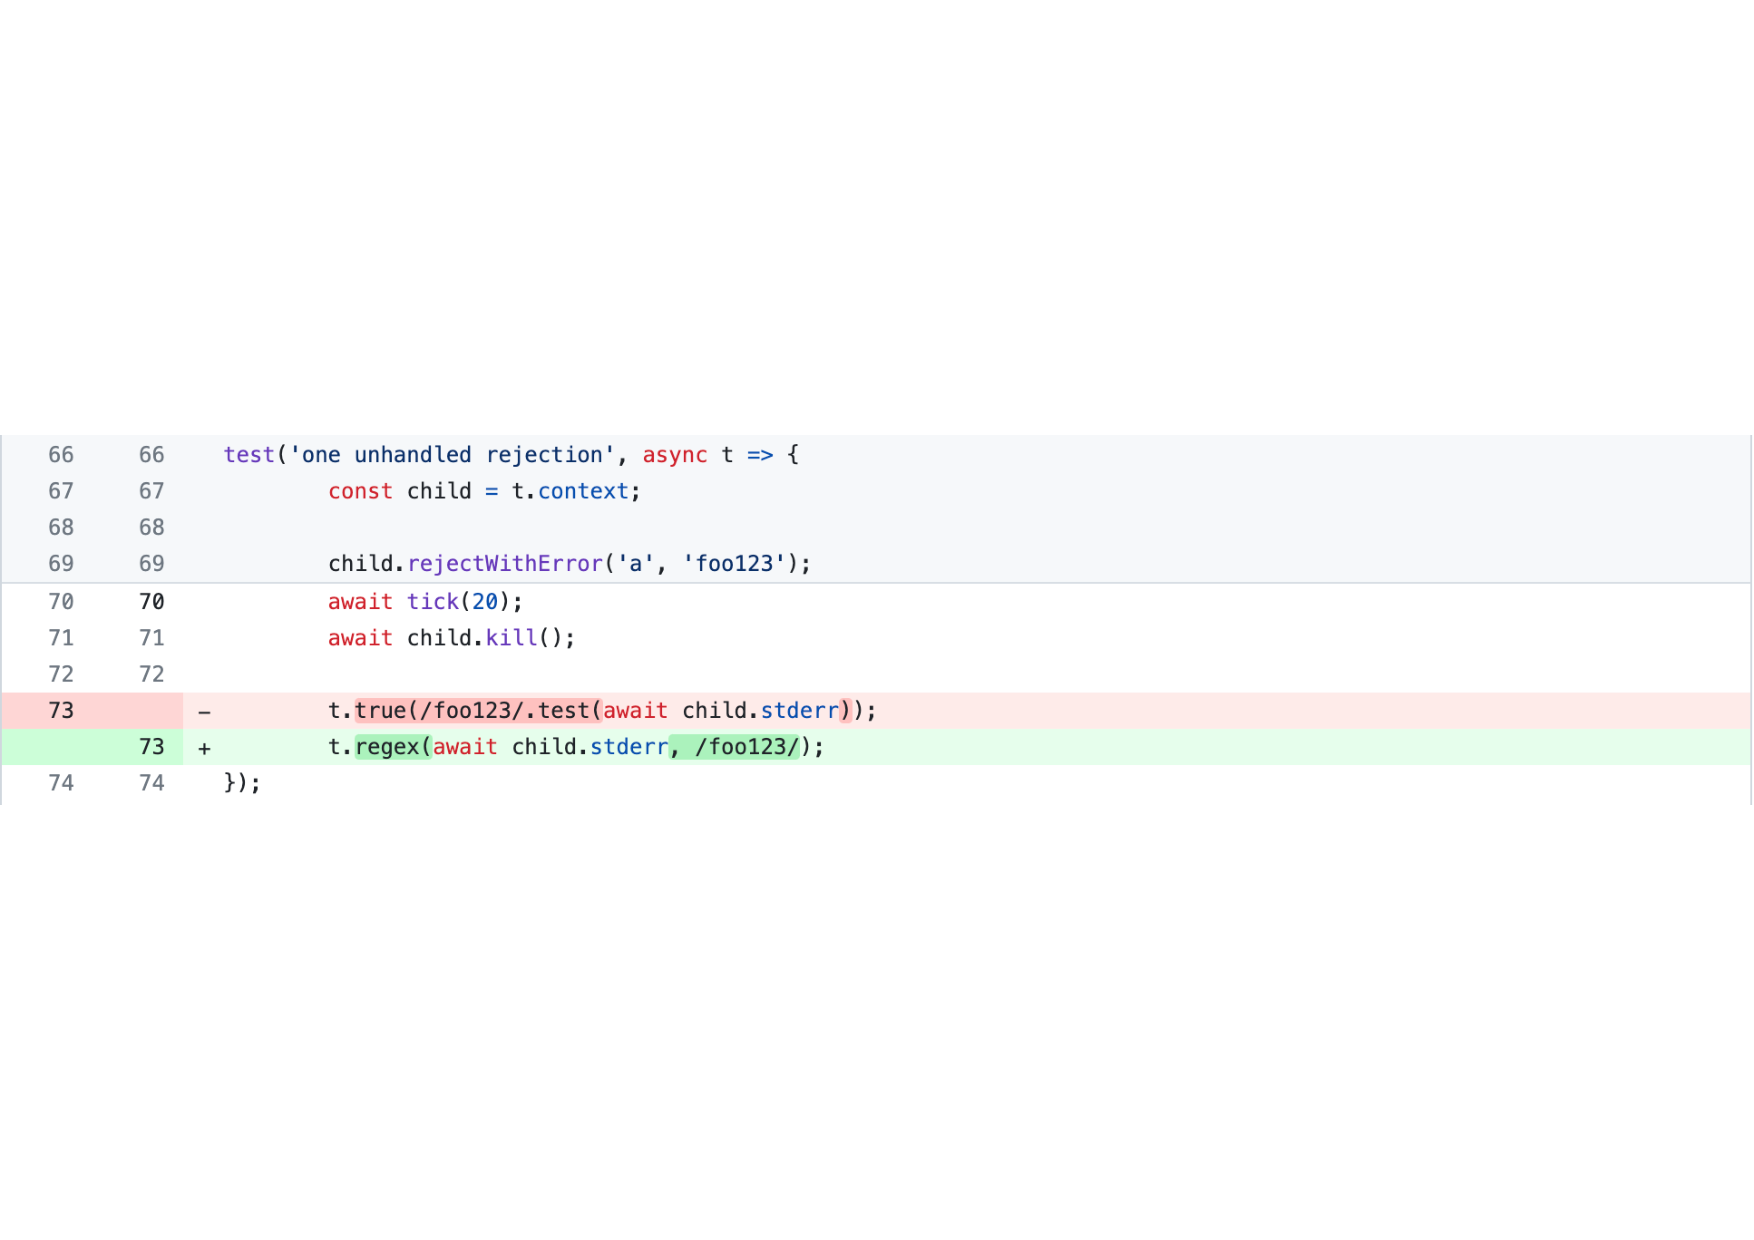
\includegraphics[width=1.0\linewidth]{fig/rq1/rejection/rejection-test.pdf}
  \caption{loud-regectionのバージョン1.2.1から1.3.0のテストコード変更差分}
  \label{fig:rq1.change-test-rejection-test}
\end{figure}

\begin{figure}[t]
  \centering
  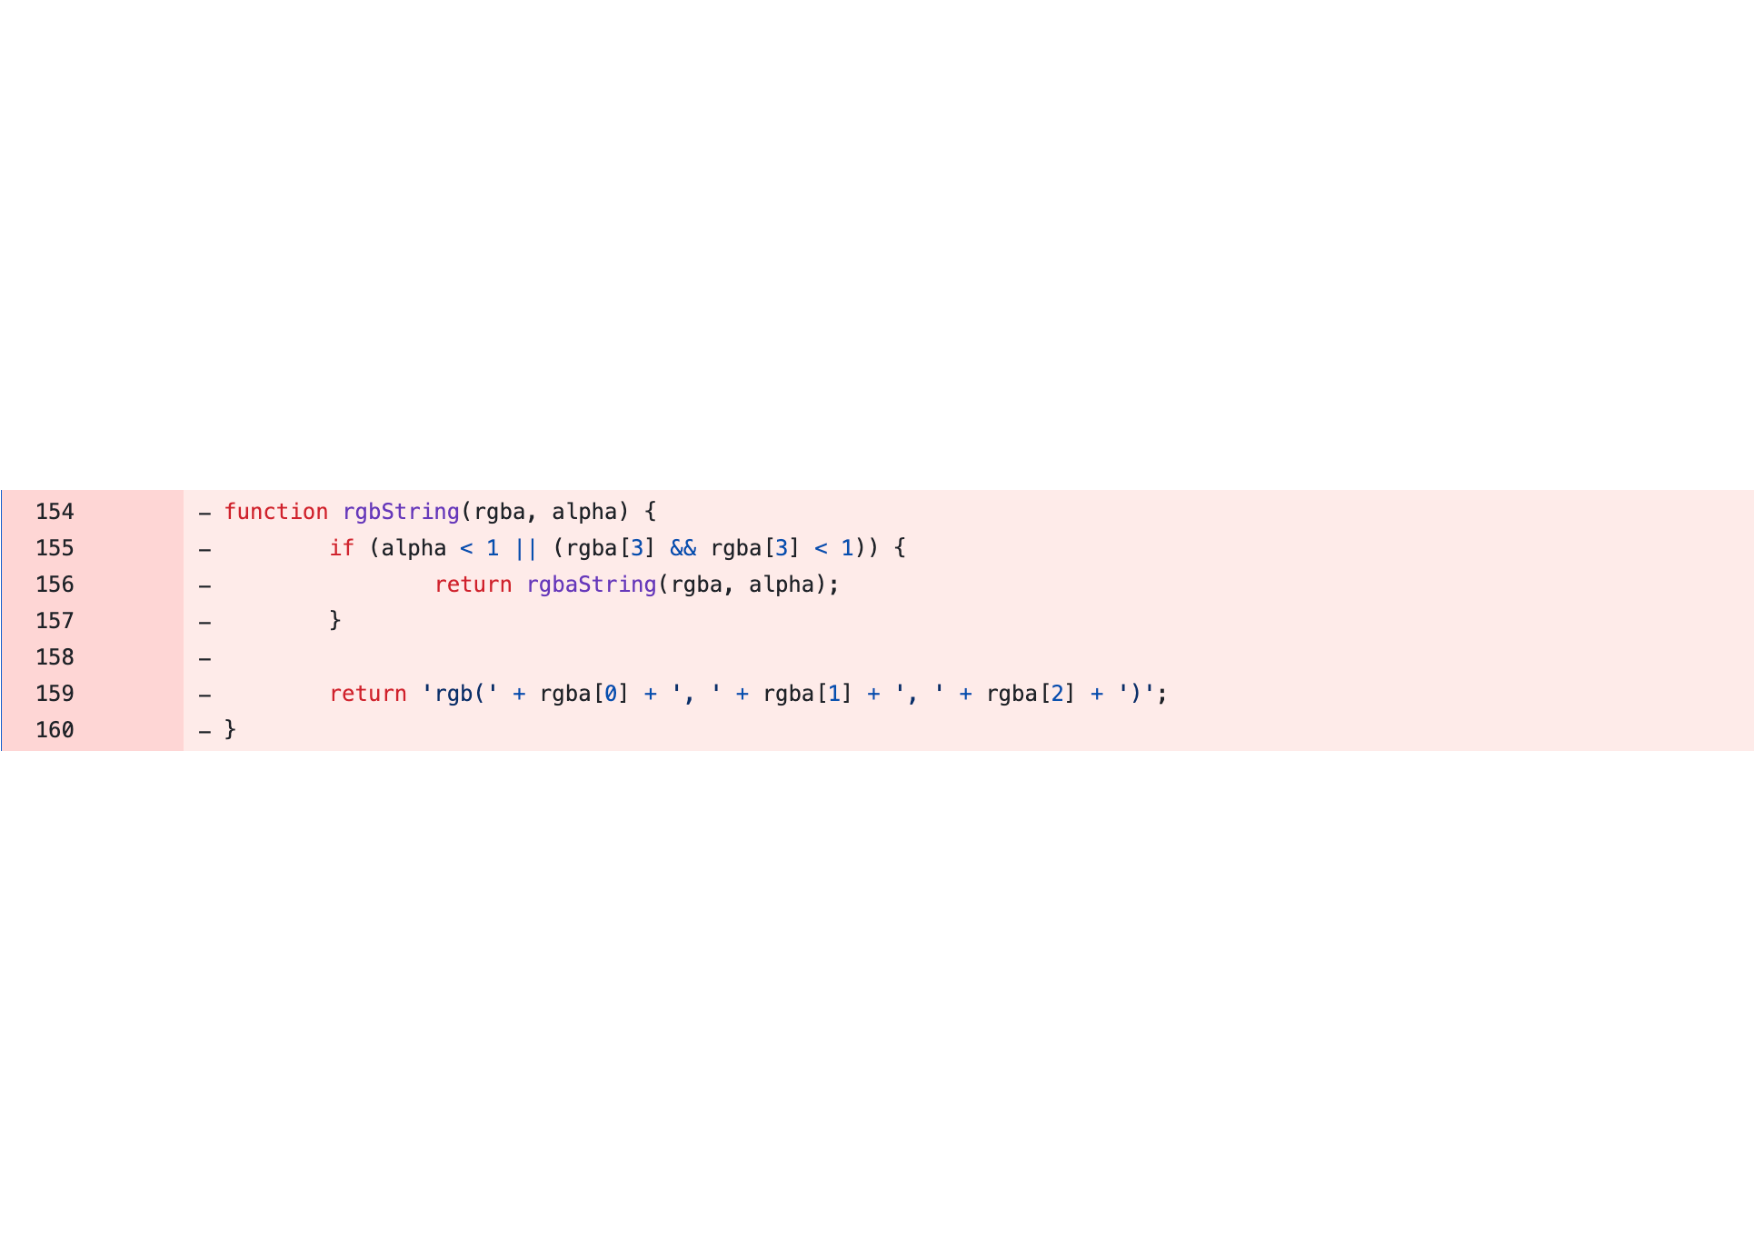
\includegraphics[width=1.0\linewidth]{fig/rq1/rgb/rgb-src.pdf}
  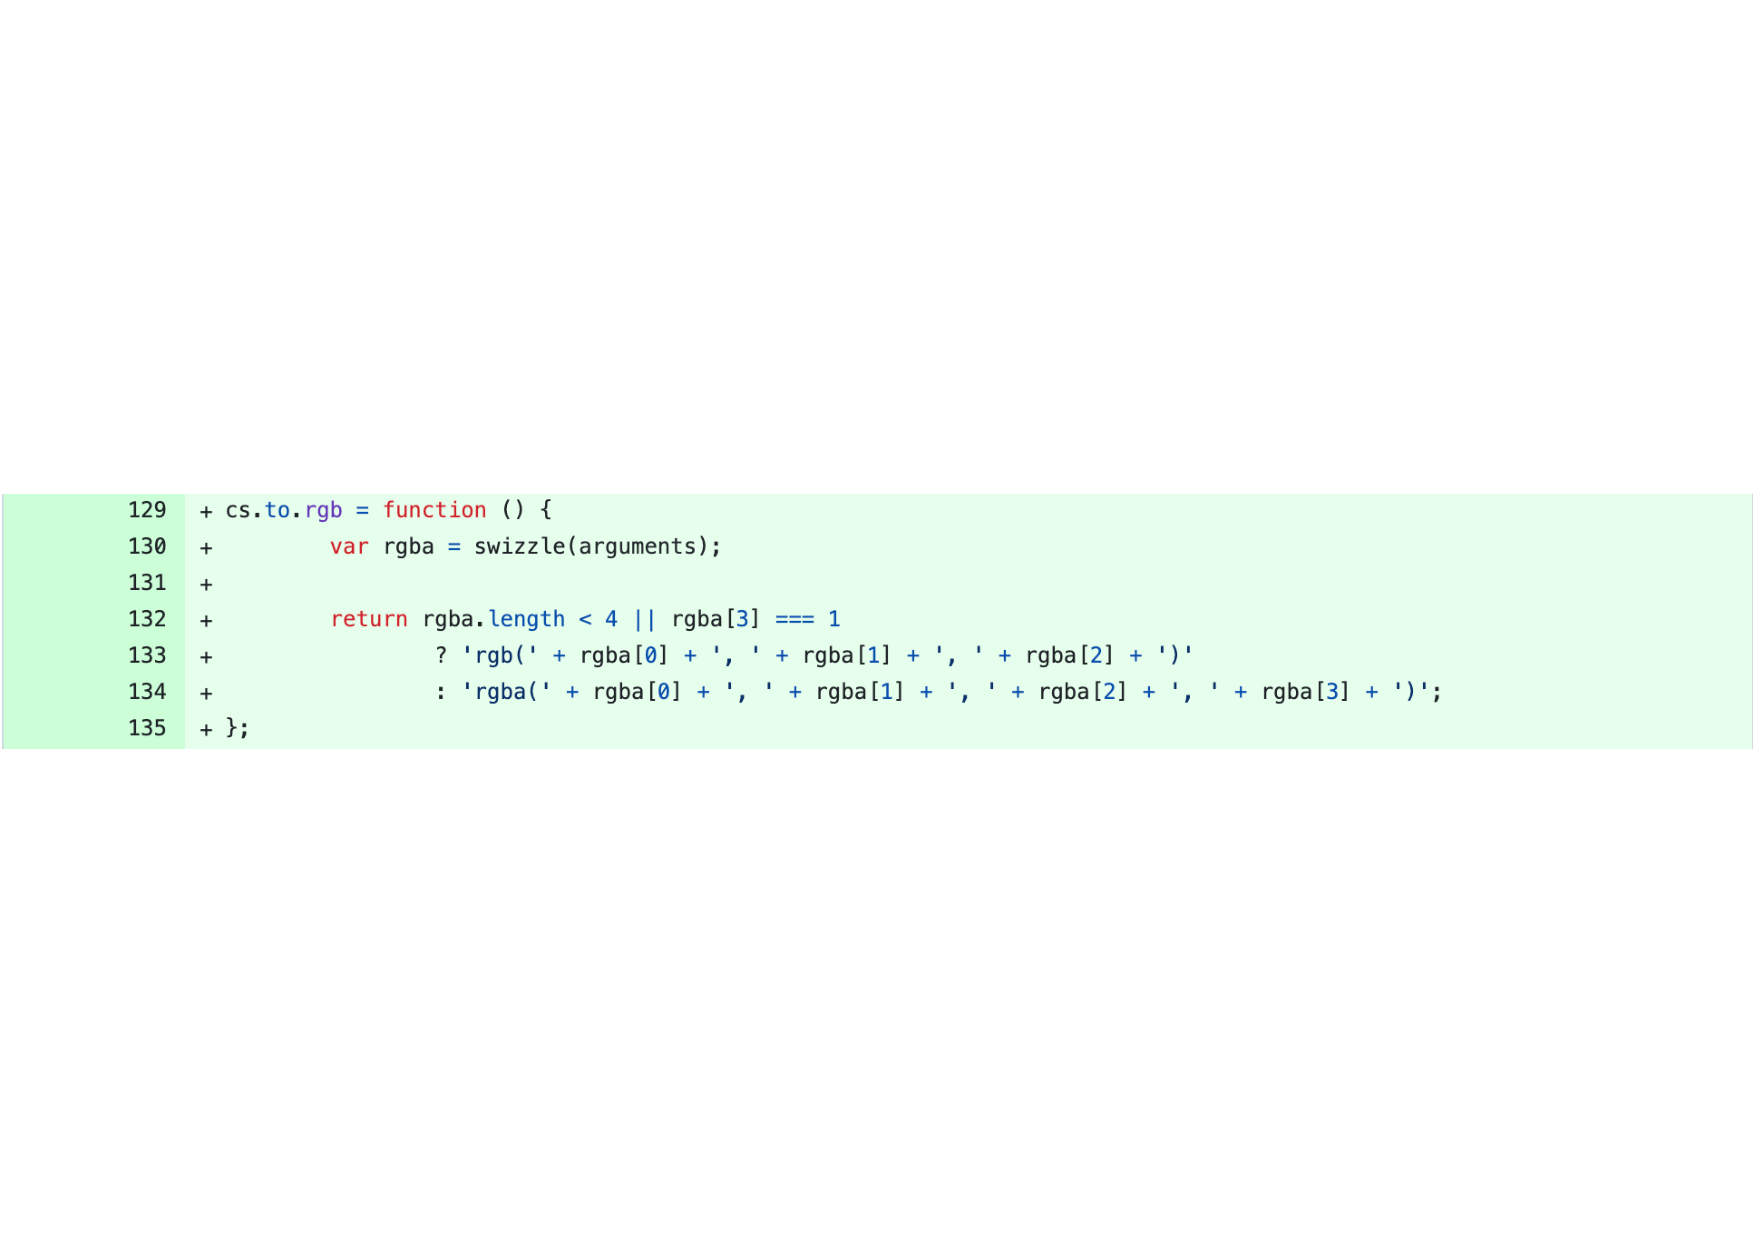
\includegraphics[width=1.0\linewidth]{fig/rq1/rgb/rgb-src-1.pdf}
  \caption{color-stringのバージョン0.4.0から1.0.0のソースコード変更差分}
  \label{fig:rq1.change-test-input-src}
\end{figure}

\begin{figure}[t]
  \centering
  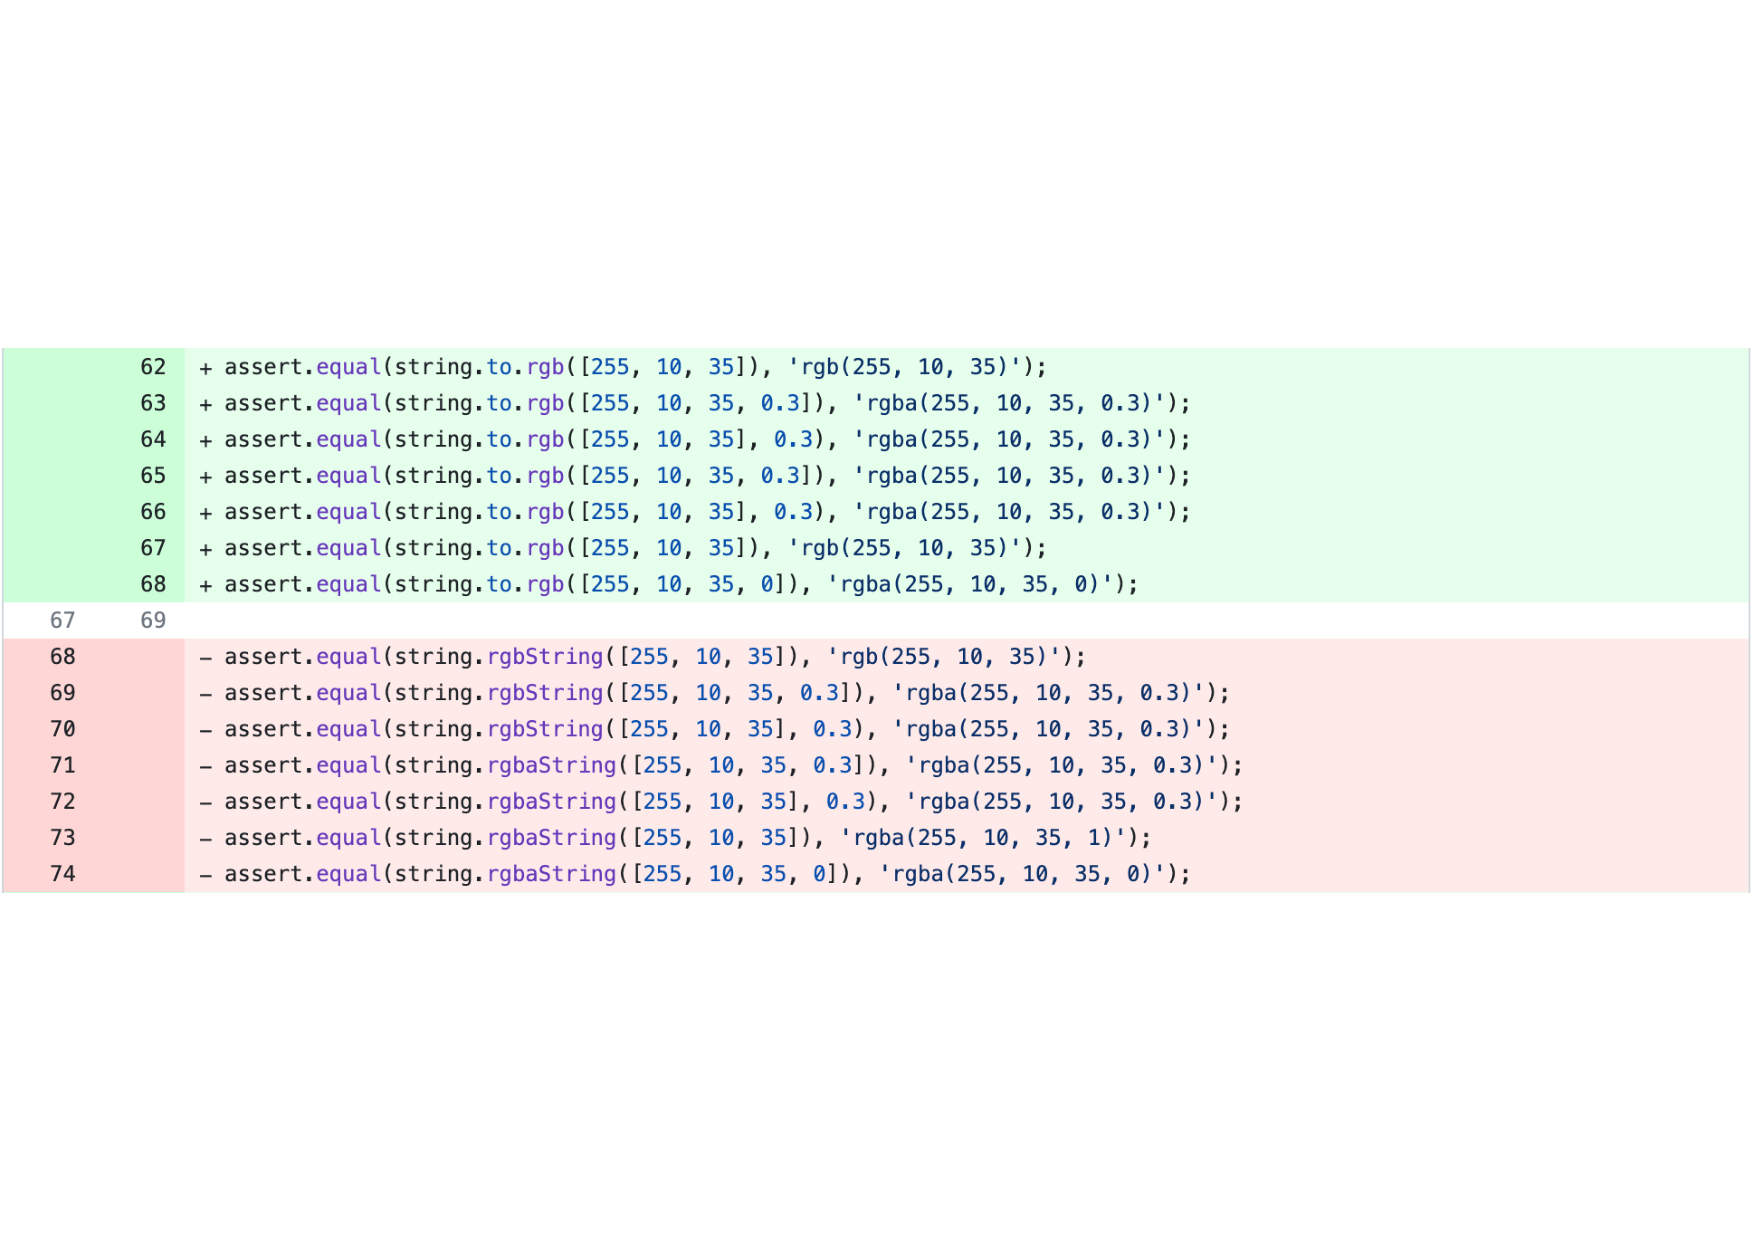
\includegraphics[width=1.0\linewidth]{fig/rq1/rgb/rgb-test.pdf}
  \caption{color-stringのバージョン0.4.0から1.0.0のテストコード変更差分}
  \label{fig:rq1.change-test-input-test}
\end{figure}

アサーションの入力値,期待値の変更やリファクタリングなどのテストコード変更は,ライブラリの更新とは無関係に行われることが多い.ライブラリの更新とは無関係にアサーションの入力値,期待値が変更される例として,非同期処理のエラー内容を追跡するAPIを提供するライブラリloud-regectionのバージョン1.2.1から1.3.0へのマイナーアップデート\footnote{\url{https://github.com/sindresorhus/loud-rejection/compare/v1.2.1...v1.3.0}}を挙げる.図\ref{fig:rq1.change-test-rejection-test}はテストコードの変更差分を示す.この変更では,アサーションメソッドを{\verb|true()|}から{\verb|regex()|}に変更しており,アサーションの入力値と期待値が同時に変更されている.ただし,テストコードの振る舞いは変わっておらず,ソースコードの変更とは無関係のテストコード変更である.一方,後方互換性を損失するライブラリ更新に伴って,アサーションの入力値,期待値が変更されることがある.アサーションの期待値が変更される例は,\ref{sec:key-idea}節で示したので割愛する.後方互換性を損失するライブラリ更新に伴ってアサーションの入力値が変更される例として,CSSの色文字列を解析するAPIを提供するライブラリcolor-stringのバージョン0.4.0から1.0.0のメジャーアップデート\footnote{\url{https://github.com/Qix-/color-string/compare/0.4.0...1.0.0}}を挙げる.図\ref{fig:rq1.change-test-input-src}はソースコードの変更差分,図\ref{fig:rq1.change-test-input-test}はテストコードの変更差分を示す.この変更では,関数{\verb|rgbString|}を{\verb|to.rgb|}に置き換えている(図\ref{fig:rq1.change-test-input-src},154行目から160行目,129行目から135行目).この変更に伴って,関数{\verb|rgbString|}に関するアサーションの入力値が変更されている.図\ref{fig:rq1.change-test-input-test}の62行目から68行目と68行目から74行目は1行ずつ対応しており,アサーションの{\verb|equal|}関数の第一引数の入力値が変更され,第二引数の期待値は変更されていない.以上から,APIの入出力形式の変更による後方互換性の損失は,アサーションの期待値もしくは入力値のいずれか一方だけ変更されるという特徴があるため,アサーションの入力値と期待値のいずれか一方が変更された場合,後方互換性を損失したと判断できると考えられる.


\section{まとめ}
本章では,後方互換性を損失するライブラリ更新に伴ってどのようなテストコード変更が行われているかを分析し,後方互換性の損失を検出する手掛かりとなるテストコード変更内容を明らかにした.結果「既存のテストスイート内でのテストコード追加」「テストコード削除」「アサーションの入力値と期待値のいずれか一方の変更」の3つが後方互換性の損失を検出する手掛かりになる,機械的に検出可能なテストコード変更であると考える.

\chapter{RQ2:テストコード変更内容に基づく後方互換性損失の検出手法の有効性はどの程度か?}\label{chap:rq2}

\section{概要}
本章では,\ref{chap:rq1}章で述べた,後方互換性を損失するライブラリ変更に伴うテストコード変更内容である「既存のテストスイート内でのテストコード追加」「テストコード削除」「アサーションの入力値と期待値のいずれか一方の変更」を自動検出するツールを開発し,後方互換性の損失の検出精度を従来手法と比較検証する.まず,変更前後のソースファイルからプログラムの変更箇所と,その変更箇所の変更方法(追加・削除など)を分類する.その後,変更箇所とその変更方法が条件に一致すれば後方互換性を損失したと判定する.

\section{提案手法}\label{sec:rq2.teian}

本研究が提案する自動検出ツールは,入力を全てのソースファイル,出力を後方互換性の有無の予測とする.まず,入力として与えられた変更前後の全てのソースファイルから,変更されていないファイルを除外し,テストコードが記述されたファイルを抽出する.従来研究\cite{matsuda}では,テストコードが記述されたファイルの条件を,ファイルパスに{\verb|test|}または{\verb|spec|}を含み,ファイル名の末尾が{\verb|.js|}または{\verb|.ts|}であるファイルとする.本研究ではこの条件に加え,ファイル名の末尾が{\verb|.d.ts|}でないファイルを条件とする.ファイル名の末尾が{\verb|.d.ts|}であるファイルは型定義ファイルであり本研究では除外する.次に,抽出したソースファイルにおける,プログラムの変更箇所とその変更方法を\ref{subsec:rq2.astseisei}項の方法で特定する.最後に,プログラムの変更箇所とその変更方法が\ref{subsec:rq2.jouken}項で述べる3つの条件に1つでも一致すれば,後方互換性が損失していると判定し,いずれにも一致しなければ後方互換性を維持していると判定する.

\subsection{プログラムの変更箇所と変更方法の特定}\label{subsec:rq2.astseisei}
プログラムの変更箇所と変更方法の特定のために,差分解析ツールであるGumTree\cite{gumtree}を使用する.GumTreeは,ソースコードの構造を表す木構造データ(抽象構文木)を基にした差分解析ツールである.構造単位で比較するため,行単位の差分解析に比べて細かい変更箇所の特定が可能になる.また,他の抽象構文木(以降,AST)を基にした差分解析ツール\cite{diff-1}\cite{diff-2}\cite{diff-3}と比べて精度が高く,JavaやJavaScriptなど複数のプログラミング言語に対応している.GumTreeは,変更前後のソースファイルまたはASTを受け取ると,それらを比較してASTのノード単位の編集操作を出力する.検出できる編集操作は,「削除」「挿入」「移動」「変更」である.ただし,GumTreeはファイル単位の差分しか検出することができず,ファイルを横断するソースコードの移動操作に対して「移動」ではなく「削除と挿入」として出力されてしまう.ファイルを横断するテストコードの移動はリファクタリングにおいて一般的に行われるため誤検出の原因となる.本手法では,藤本らの手法\cite{gumtreenoyatu}を一部利用し,次の手順で複数ファイルを横断してGumTreeを適用する.

\begin{enumerate}
  \setlength{\itemsep}{0cm}
  \item 変更のある各ファイルごとにASTを生成する
  \item 根となるノードを1つ作成する
  \item 各ファイルごとに生成したASTを子ノードとして加えていく
  \item 1から3を変更前後で実施し,2つASTを生成する
  \item 変更前後で生成された2つのASTをGumTreeに入力して出力を得る
\end{enumerate}

この方法により,バージョン間のテストコード変更に対して,プログラムの変更箇所(ノード)と,「削除」「挿入」「移動」「変更」の4つの変更方法をファイルを横断する移動操作も含めて特定することができる.

\subsection{後方互換性を損失したバージョンの判定条件}\label{subsec:rq2.jouken}
\ref{chap:rq1}章で述べた,「既存のテストスイート内でのテストコード追加」「テストコード削除」「アサーションの入力値と期待値のいずれか一方の変更」を自動で検出するために,それぞれ条件を定義する.

まず,「既存のテストスイート内でのテストコード追加」「テストコード削除」を判定するために,テストコードを定義する.従来研究\cite{matsuda}では,テストファイル内に記述されている,関数名が{\verb|it|}または{\verb|test|}である関数呼び出しをテストケースとしている.本研究では,テストスイートの追加・削除を含めるため,慣習的にテストスイートの宣言として使われる関数名{\verb|describe|}を加え,{\verb|it|}または{\verb|test|}または{\verb|describe|}のいずれかの関数呼び出しで,第一引数が文字列,第二引数が関数であるものをテストスイートまたはテストケースと定義する.

次に,「アサーションの入力値と期待値のいずれか一方の変更」を判定するために,アサーションの入力値と期待値を定義する.JavaScript言語では,アサーションの書き方はフレームワークによって異なる.本手法では,State of JavaScript 2022\footnote{\url{https://2022.stateofjs.com/}}で紹介されている主要なテストフレームワーク13件のうち,単体テストで使われるフレームワーク5件(Jest\footnote{\url{https://jestjs.io/}},Mocha\footnote{\url{https://mochajs.org/}},AVA\footnote{\url{https://github.com/avajs/ava}},Jasmine\footnote{\url{https://jasmine.github.io/}},Vitest\footnote{\url{https://vitest.dev/}})を対象とする.Mochaは複数のアサーションの記述スタイルを利用できるため,Mochaで使用可能なアサーションのスタイルについても対象とする.テストフレームワーク毎のアサーションの書き方は,大きく2つに大別できる.例をProgram\ref{bdd.test.js},Program\ref{tdd.test.js}で示す.

\begin{lstlisting}[caption=アサーション例1, label=bdd.test.js]
expect(calculator.add(1, 1)).to.be.a('number').equal(2);
expect(calculator.add(1, 1), 'to be', 2);
calculator.add(1, 1).should.be.a('number').equal(2);
\end{lstlisting}

Program\ref{bdd.test.js}は,自然言語に似た構文を使用してテストを記述する記述形式で,Jest,Mocha,Jasmine,Vitestで使用される.その中でも,1行目のように,{\verb|expect|}関数にメソッドチェーンで振る舞いを記述する形式,2行目のように{\verb|expect|}関数の引数にそのまま振る舞いを記述する形式,3行目のように入力値に{\verb|should|}プロパティを追加して振る舞いを記述する形式がある.1,2行目の形式に対しては,{\verb|expect|}関数の第一引数を入力値,それ以降を期待値として扱い,3行目の形式に対しては,{\verb|should|}プロパティ以前を入力値,以降を期待値として扱う.

\begin{lstlisting}[caption=アサーション例2, label=tdd.test.js]
assert.equal(calculator.add(1, 1), 2);
t.is(calculator.add(1, 1), 2);  
t.true(calculator.add(1, 1) === 2);
\end{lstlisting}

Program\ref{tdd.test.js}は,Node.js\footnote{\url{https://nodejs.org/en}}標準の{\verb|assert|}文がメインの記述形式で,AVA,Mochaで使用される.その中でも,1行目や2行目のように,第一引数に入力値,第二引数に期待値を取る形式と,3行目のように入力だけを引数に取る形式がある.この記述形式に対しては,{\verb|assert|},{\verb|t|},{\verb|test|}をキーとして,アサーションメソッドの第一引数を入力,第二引数を期待値として扱う.3行目のように引数が1つの場合は,引数を入力,アサーションメソッド名を期待値とする.

これらのテストコードの定義を利用し,後方互換性を損失するライブラリ更新に伴うテストコード変更内容である,「既存のテストスイート内でのテストコード追加」「テストコード削除」「アサーションの入力値と期待値のいずれか一方の変更」を検出する3つの条件を定める.

\begin{description}
  \item[\textbf{既存のテストスイート内でのテストコード追加}]:GumTreeで「挿入」と判定された変更箇所がテストコードまたはアサーションであり,かつ既存のテストコード内で追加されていること
  \item[\textbf{テストコード削除}]:GumTreeで「削除」と判定された変更箇所がテストコードであること
  \item[\textbf{アサーションの入力値と期待値のいずれか一方の変更}]:GumTreeで「変更」と判定された変更箇所がアサーションの入力値もしくは期待値であり,同一アサーションの入力値もしくは期待値がGumTreeで「変更」と判定されていないこと
\end{description}

ライブラリバージョンに含まれるテストコード変更内容が,以上3つの条件に1つでも当てはまれば,ライブラリバージョンは後方互換性を損失したと判定し,1つも当てはまらなければライブラリバージョンは後方互換性を維持したと判定する.

\section{データセット}
データセットは,\ref{rq1:datasets}節と同様の従来研究\cite{matsuda}で収集されたライブラリバージョン2,111件を使用し,削除や非公開になったことによりGitHub上でアクセスできないものと,GumTree上でエラーになるもの計156件を除いた1,955件を使用する.

\section{分析結果}

\begin{table}[t]
\centering
\caption{提案手法と従来手法の比較結果}
\label{fig:result}
\begin{tabular}{cl|r|r|r}
\hline
\multicolumn{2}{c|}{} & \multicolumn{1}{c|}{後方互換性なし} & \multicolumn{1}{c|}{後方互換性あり} & \multicolumn{1}{c}{合計} \\ \hline
\multicolumn{1}{c|}{\multirow{3}{*}{提\newline 案\newline 手\newline 法}} & 後方互換性なしと判定      & 114 & 548 & 662 \\ \cline{2-5} 
\multicolumn{1}{c|}{}                                                      & 後方互換性ありと判定      & 109 & 1,184 & 1,293 \\ \cline{2-5} 
\multicolumn{1}{c|}{}                                                      & 合計              & 223 & 1,732 & 1,955 \\ \hline
\multicolumn{1}{c|}{\multirow{3}{*}{従\newline 来\newline 手\newline 法}} & 従来手法で後方互換性なしと判定 & 140 & 765 & 905 \\ \cline{2-5} 
\multicolumn{1}{c|}{}                                                      & 従来手法で後方互換性ありと判定 & 83  & 967 & 1,050 \\ \cline{2-5} 
\multicolumn{1}{c|}{}                                                      & 合計              & 223 & 1,732 & 1,955 \\ \hline
\end{tabular}
\end{table}

データセットに対して,従来手法と\ref{sec:rq2.teian}節で述べた手法を適用した結果を表\ref{fig:result}に示す.分析対象とするライブラリバージョン1,955件中,提案手法で後方互換性なしと判定したライブラリバージョンは662件(約34%),後方互換性ありと予測したライブラリバージョンは1,293件(約66%)であった.また,従来手法で後方互換性なしと予測したライブラリバージョンは905件(約46%),後方互換性ありと予測したライブラリバージョンは1,050件(54%)であった.

提案手法で後方互換性を損失したと判定したライブラリバージョン662件中,114件(約17%)は後方互換性を損失し(適合率),662件中548件(約83%)は後方互換性を維持している.また,後方互換性を損失したライブラリバージョン223件中,114件(約51%)を正しく予測した(再現率).従来手法では,後方互換性を損失したと予測したライブラリバージョン905件中,140件(約15%)が後方互換性を損失(適合率)し,後方互換性を損失したライブラリバージョン223件中,140件(63%)を正しく予測した(再現率).

従来手法では,後方互換性を維持するライブラリバージョンに対し,後方互換性を損失したと誤検出した件数は765件であり,提案手法は548件が誤検出であった.これは,従来手法で誤検出となる,テストケースの移動やラベルの修正などのテストコードのリファクタリングによる影響を提案手法では受けないため,誤検出を減らすことができたことを示している.一方で,提案手法は従来手法に比べて,後方互換性を損失したライブラリバージョンの検出精度が低下している.従来手法では後方互換性を損失したライブラリバージョン223件中,140件を正確に検出できたのに対し.提案手法では114件のみを検出した.この結果から,提案手法は誤検出を減らすことには成功しているが,後方互換性を損失したライブラリバージョンの検出においては改善の余地があるとわかる.予測結果を目視により調査した内容については,\ref{rq2:kousatu}章で言及する.


\section{考察}\label{rq2:kousatu}

分析したライブラリバージョンを目視で確認し,ライブラリバージョンの例を挙げて分析結果について考察する.

\subsection{従来手法と提案手法の検出精度}

\begin{figure}[t]
  \centering
  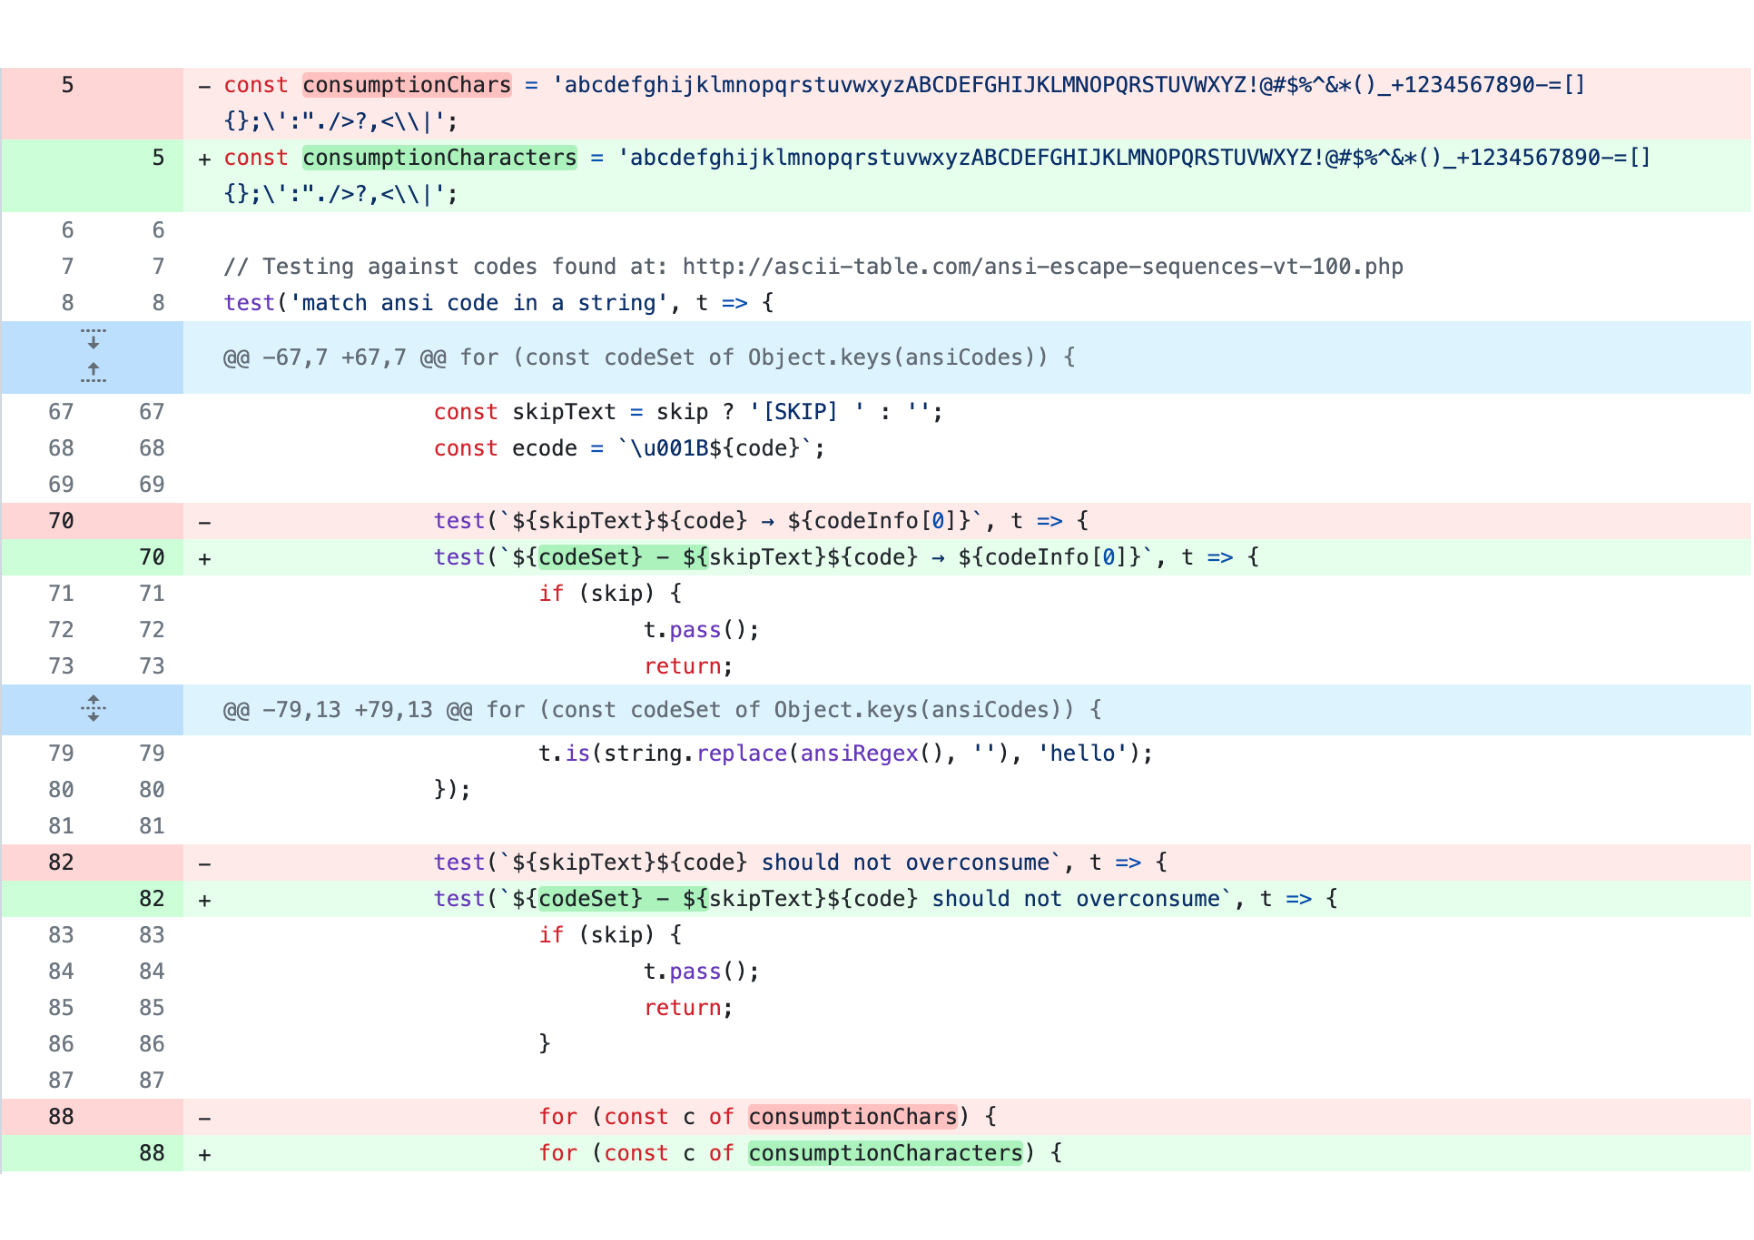
\includegraphics[width=1.0\linewidth]{fig/rq2/ansi-regex.pdf}
  \caption{ansi-regexのバージョン4.1.0から5.0.0のテストコード変更差分}
  \label{fig:rq2.ansi-regex}
\end{figure}

\begin{figure}[t]
  \centering
  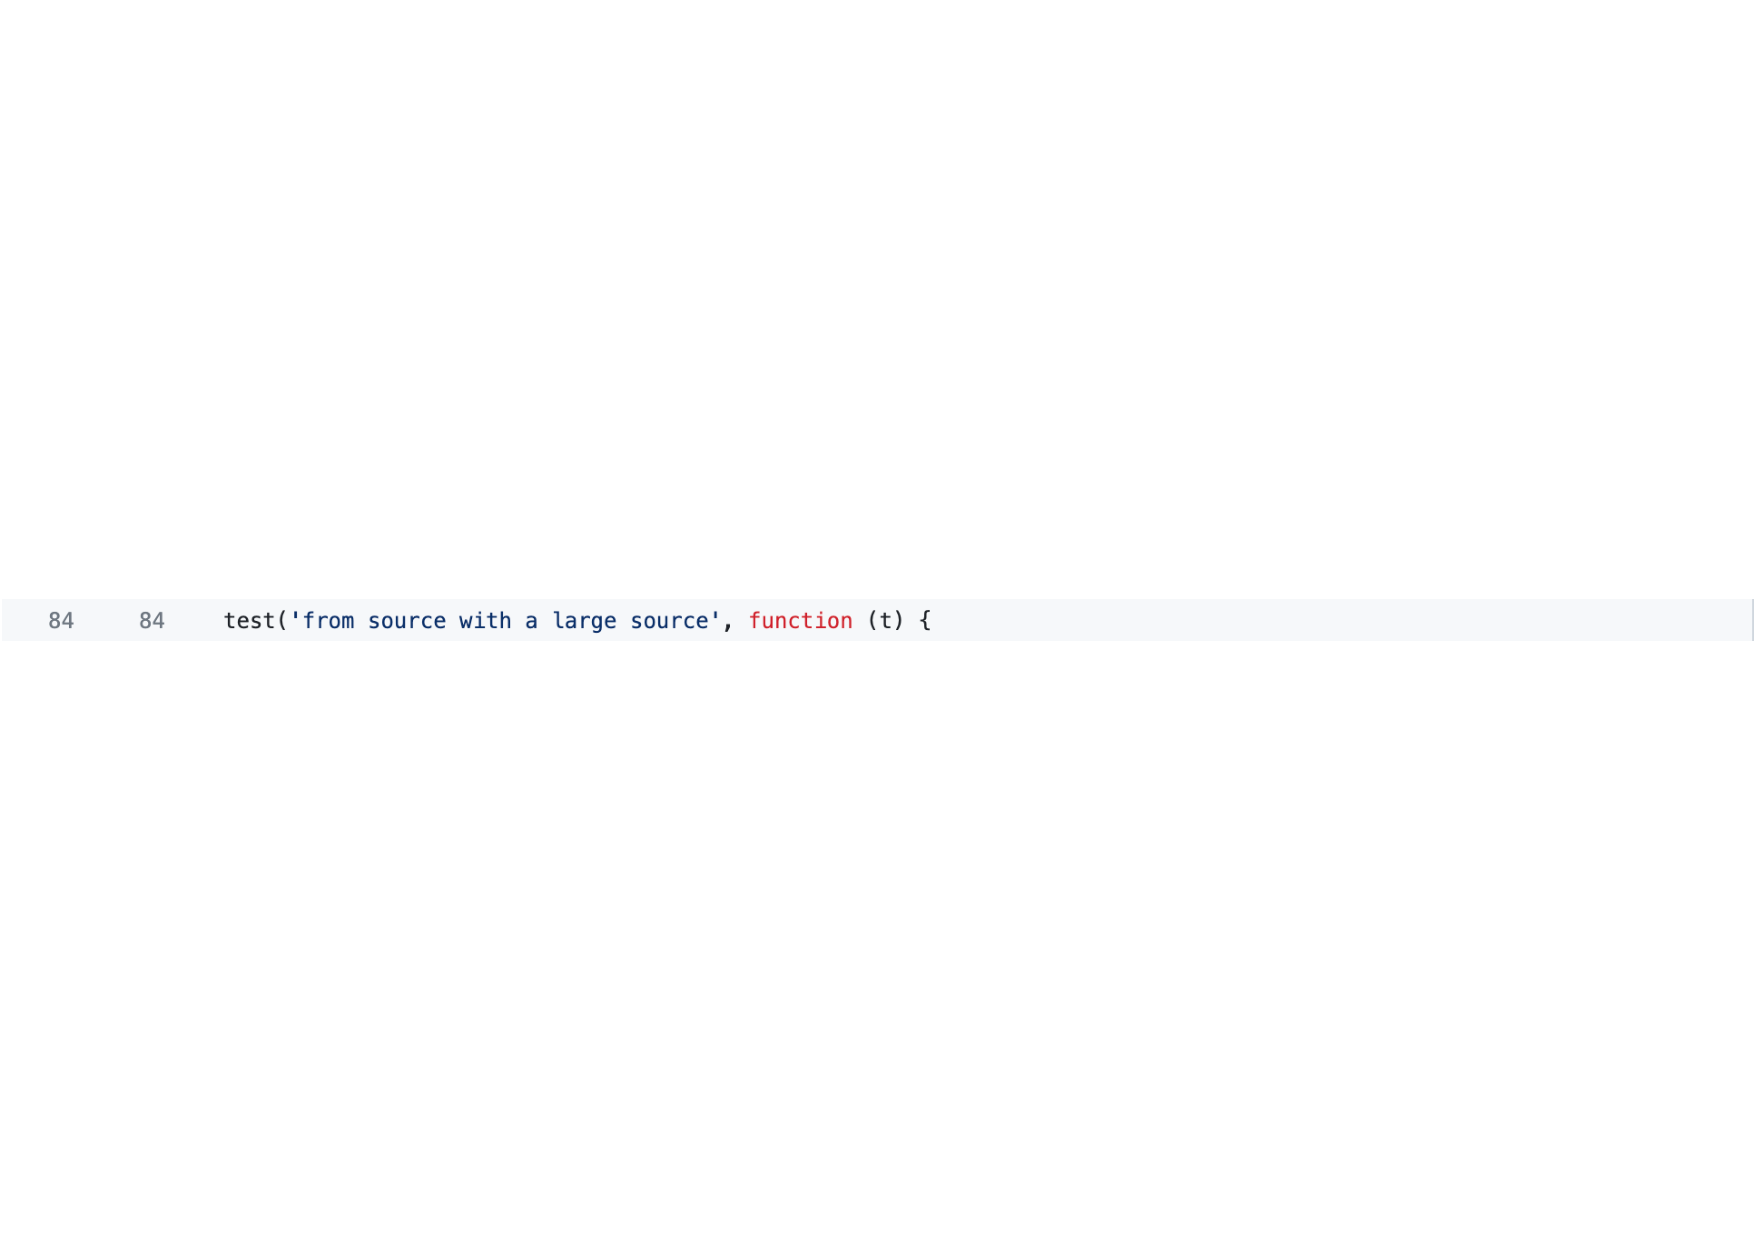
\includegraphics[width=1.0\linewidth]{fig/rq2/source-map-1.pdf}
  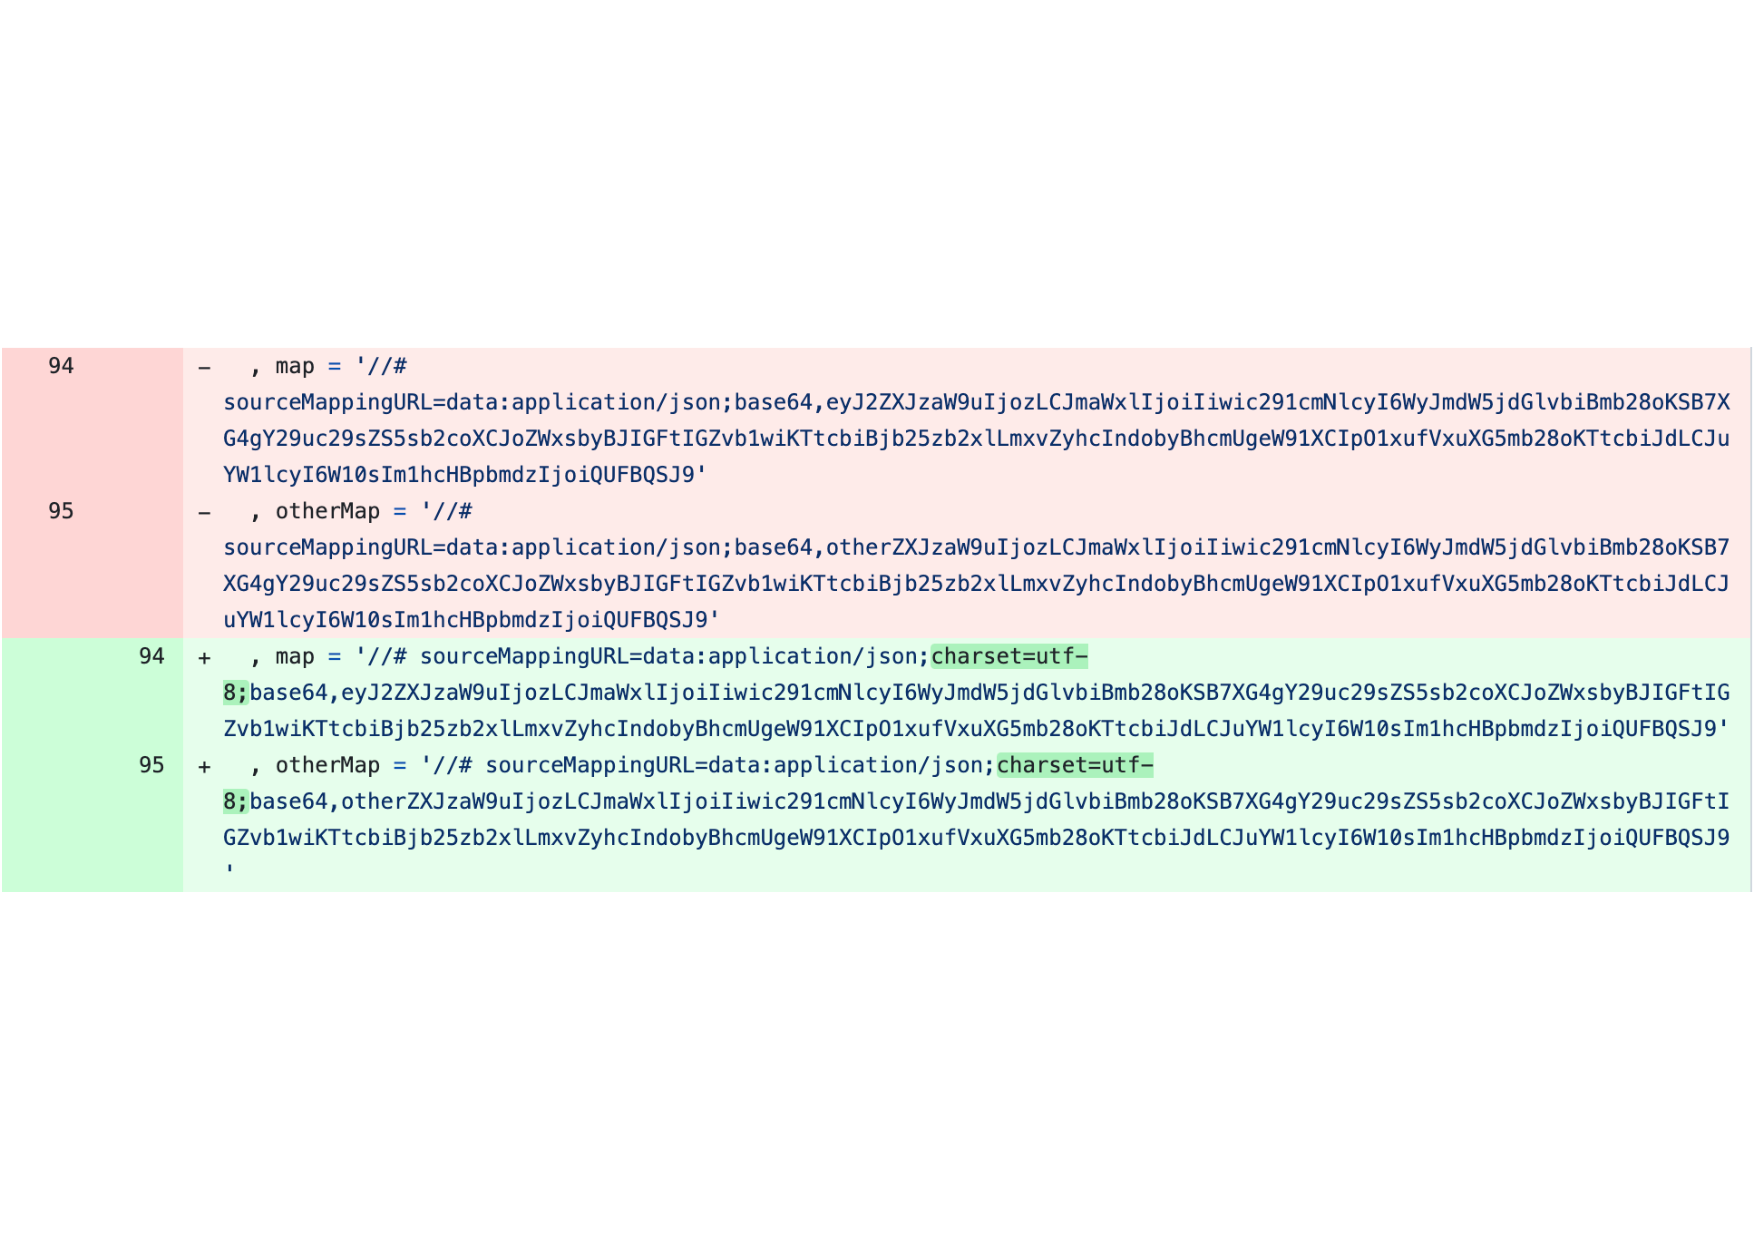
\includegraphics[width=1.0\linewidth]{fig/rq2/source-map-2.pdf}
  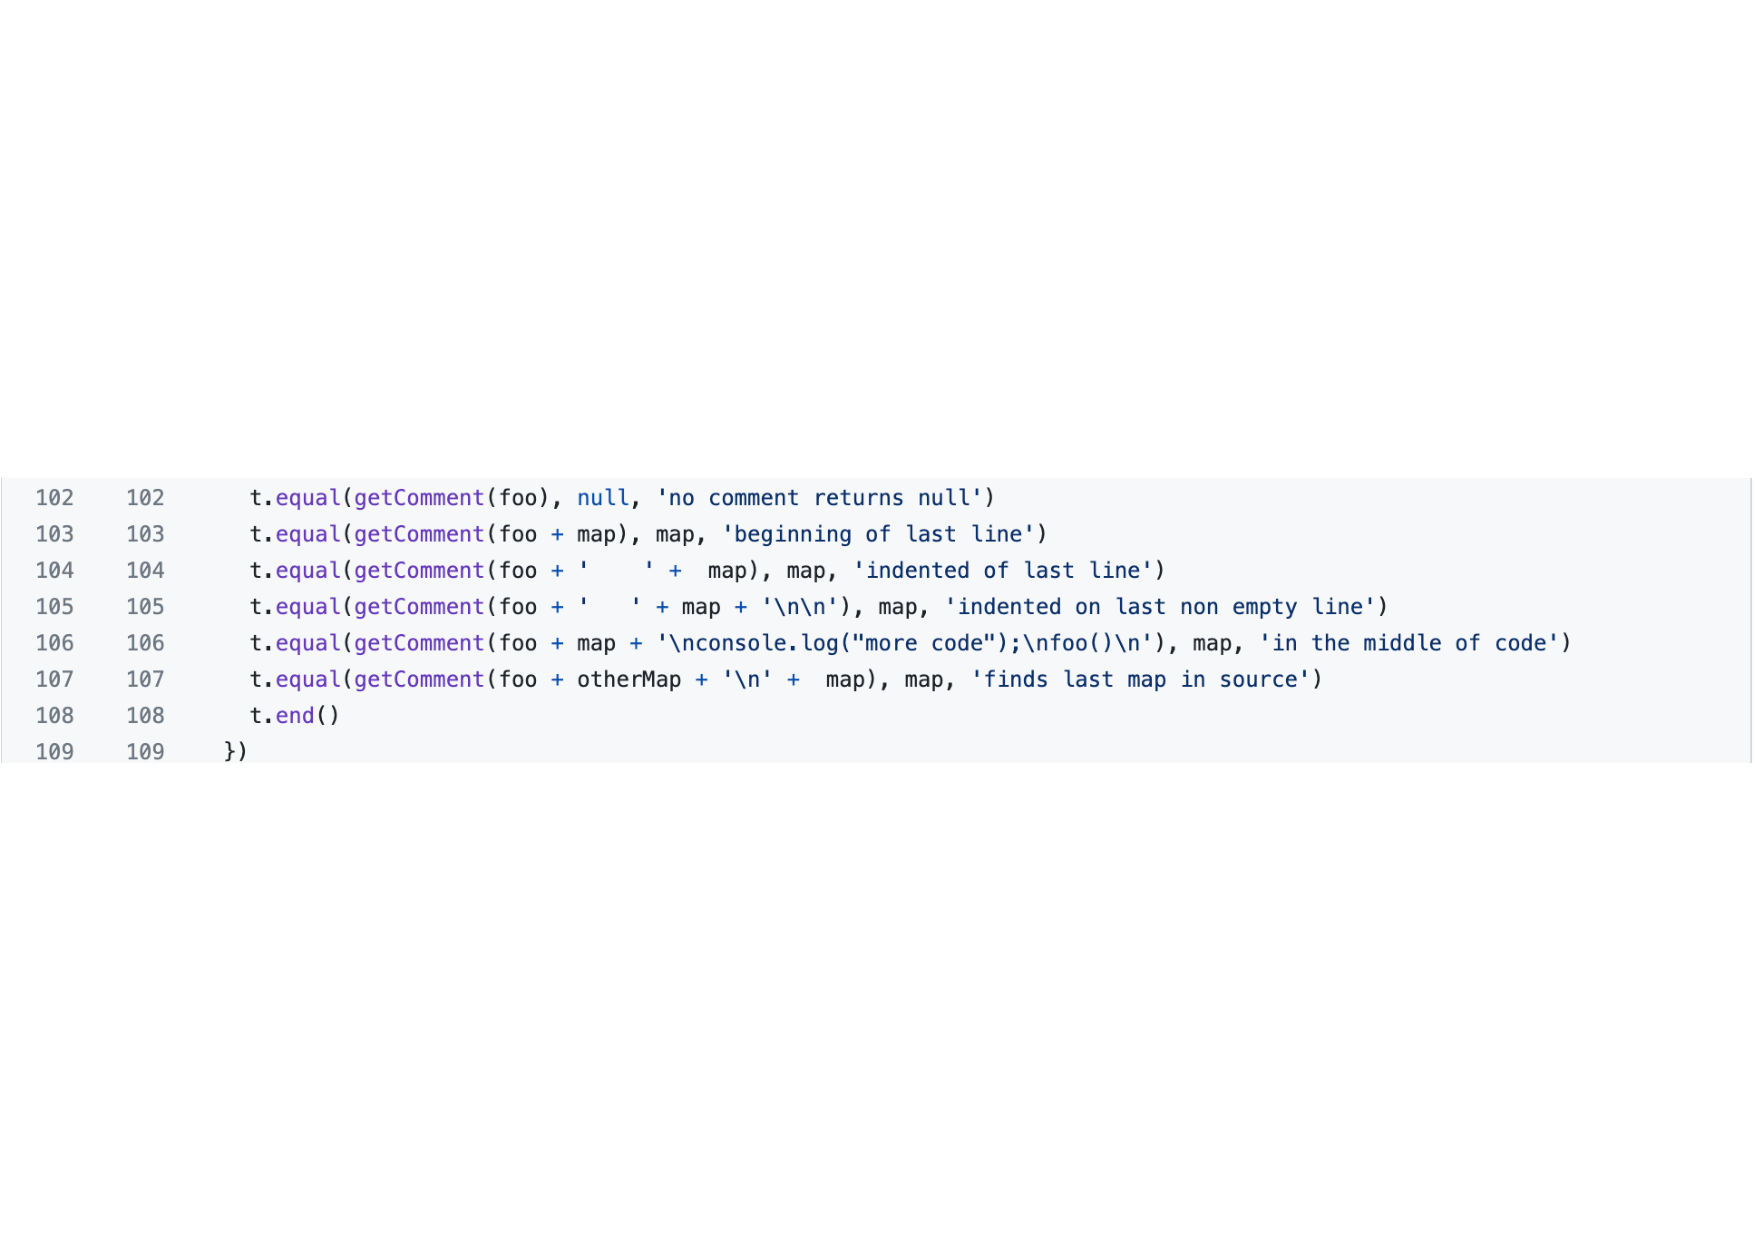
\includegraphics[width=1.0\linewidth]{fig/rq2/source-map-3.pdf}
  \caption{convert-source-mapのバージョン1.3.0から1.4.0のテストコード変更差分}
  \label{fig:rq2.convert-source-map}
\end{figure}

提案手法のライブラリの後方互換性損失の検出精度が従来手法より低下した原因を考察する.精度低下の原因として,後方互換性を損失したと判定する条件を絞り込んだことが考えられる.従来手法では,テストコードの任意の変更を後方互換性の損失を判定する指標としていたため,より多くのライブラリバージョンを後方互換性を損失したと判定する.しかし,従来手法のアプローチは後方互換性の有無の状況を正確に反映していないことがある.例として,コマンドライン出力などで使用されるANSIコードを識別するAPIを提供するライブラリansi-regexのバージョン4.1.0から5.0.0のメジャーアップデート\footnote{\url{https://github.com/chalk/ansi-regex/compare/v4.1.0...v5.0.0}}を挙げる.図\ref{fig:rq2.ansi-regex}はテストコードの変更差分を示す.この変更では,サポートするNode.jsのバージョン更新など,メジャーアップデートであることからもわかる通り後方互換性を損失する変更を含む.一方,テストコード変更差分は,図\ref{fig:rq2.ansi-regex}で示すように,テストコードのラベルの変更(70行目)や変数名の変更(5行目)によるリファクタリングに留まっている.従来手法では,テストコード変更内容を考慮しないため後方互換性を損失したと判定するが,提案手法ではテストコード変更内容を考慮するため,例のように後方互換性の損失とテストコード変更内容が無関係である場合検出することはできない.従来手法の検出精度は,ライブラリ本体の変更とテストコードの変更の関連性を十分に評価していないことに起因し,提案手法の検出精度の低下は,後方互換性を損失したと判定する条件を絞り込んだ結果と解釈できる.

次に,\ref{subsec:rq2.jouken}項で定義した条件では,検出すべきテストコード変更内容を検出できなかったことが考えられる.例として,異なるフォーマットのソースマップを相互に変換するAPIを提供するライブラリconvert-source-mapのバージョン1.3.0から1.4.0のマイナーアップデート\footnote{\url{https://github.com/thlorenz/convert-source-map/compare/v1.3.0...v1.4.0}}を挙げる.図\ref{fig:rq2.convert-source-map}はテストコードの変更差分を示す.この変更では,メモリ不足によるエラーを解消するためのフラグを追加し既存APIの機能を拡張している.テストコードは,図\ref{fig:rq2.convert-source-map}の84行目のテストケースに対して,94行目から95行目の変数{\verb|map|},{\verb|otherMap|}が変更されている.変数{\verb|map|},{\verb|otherMap|}は続く102行目以降のアサーションの入力値として使用されており,入力値が変更されているため,提案手法で検出すべきテストコード変更内容である.しかし,GumTreeを利用した差分検出のみでは変数の中身を追跡できないため,後方互換性の損失と判定することはできない.コールグラフを利用した追跡を組み合わせて検出することが考えられるが,JavaScript言語では動的な性質からコールグラフ作成は困難であるため\cite{js-call-graph},今後の課題とする.

また,後方互換性の有無のデータにはクライアントのテストコードを利用している.ライブラリの後方互換性が損失していても,影響を受けるクライアントが存在しない場合,後方互換性の損失を確認することができず,分析の精度を低下させる原因になる.今後の研究では正解データをより正確に収集し分析することが必要となる.

\subsection{提案手法の有効性}

\begin{figure}[t]
  \centering
  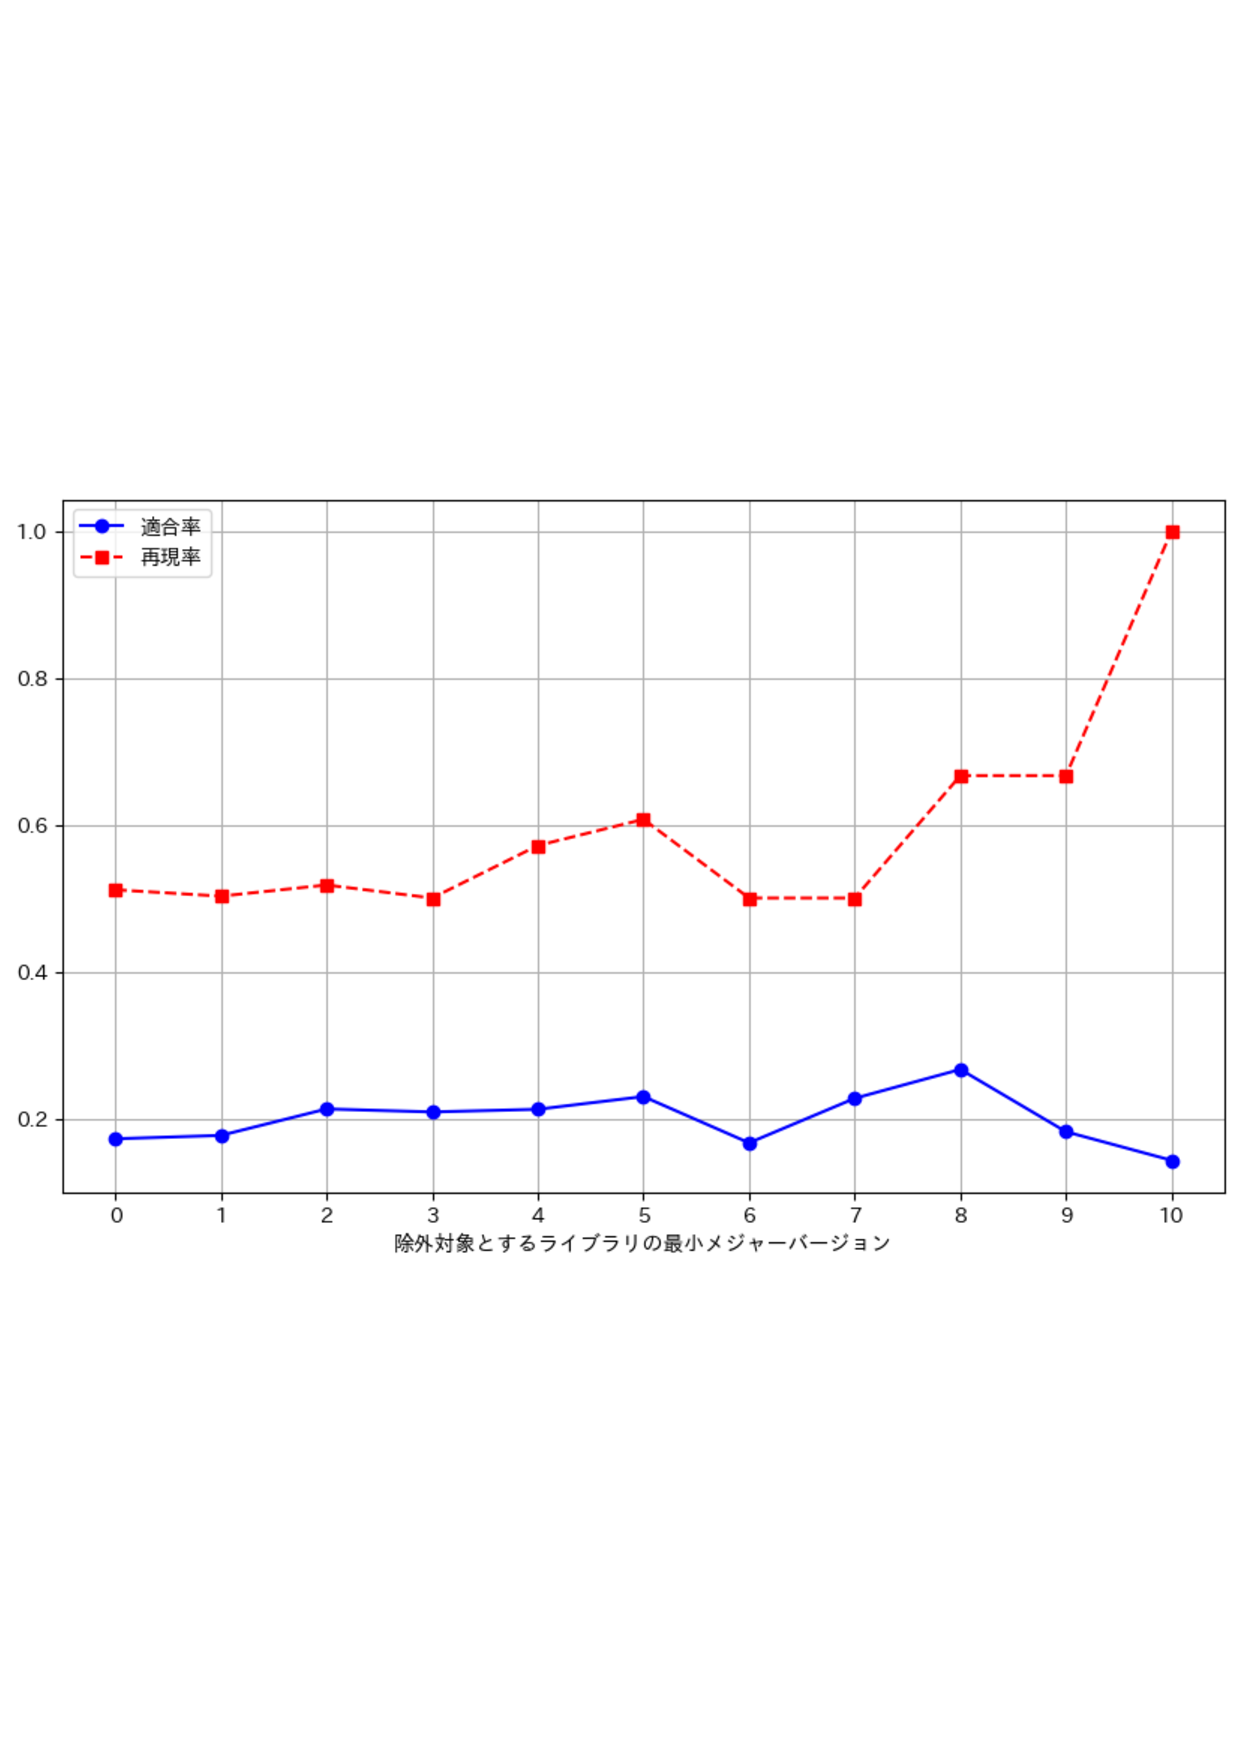
\includegraphics[width=1.0\linewidth]{fig/tuikabunseki.pdf}
  \caption{ライブラリのメジャーバージョンに基づく適合率と再現率の推移}
  \label{fig:tuikabunseki}
\end{figure}

本手法は,ライブラリの変更とテストコードの変更の関連性を考慮するため,ライブラリとテストコードが伴って変更されるような,成熟したライブラリにおいて有効である場合がある.分析対象としたライブラリバージョンから,メジャーバージョンが一定以下だったライブラリバージョンを除外した場合の結果を考察する.除外対象とするライブラリバージョンの最低メジャーバージョンを0から10(分析対象ライブラリの最大値)までとし,1ごとに適合率と再現率を計算した.結果を図\ref{fig:tuikabunseki}に示す.

再現率は,メジャーバージョンが上昇するにつれて,0.5から1.0の間で徐々に高くなる傾向が見られる.これは,メジャーバージョンが高く,成熟したライブラリでは,後方互換性が損失するライブラリ更新に伴ってテストコードが変更される可能性が高いことを示している.つまり,成熟したライブラリの開発者は,後方互換性のない変更をより慎重に扱い,それに伴うテストコードの更新を行う傾向があると考えられる.一方で,適合率は0.1から0.3の範囲で推移しており,比較的低い値を示している.適合率が低い理由として,分析対象となるライブラリのクライアント数が少なく,後方互換性の損失を確認することができなかったことが考えられる.

\section{まとめ}
本章では,後方互換性の損失に伴うテストコード変更内容を自動検出するツールを開発し,後方互換性の判定精度を従来手法と比較検証した.分析結果から,提案手法は従来手法に比べて,後方互換性を維持しているライブラリバージョンに対し,後方互換性を損失したと誤検出する件数を減らすことができた.一方で,後方互換性を損失したライブラリバージョンの検出においては,提案手法の精度が従来手法の精度より低下していることがわかった.これは,提案手法が後方互換性を損失したと判定する条件を絞ったため,検出件数が減少し,結果として精度が低くなったと考えられる.また,後方互換性の判定精度の検証には,クライアントのテストコードの分析が重要であると再確認された.不十分なクライアントのテストコードは,正解データの質に影響を与え,分析の精度を低下させるため,今後の研究では正解データをより正確に収集し分析することが必要である.

\chapter{妥当性の脅威}\label{chap:heuristic}
\section{内的妥当性}
\ref{chap:rq1}章の分析では,テスト変更内容を著者が目視により分類した.著者は一定のソフトウェア開発経験を有しているが,結果は著者の主観に依存する.目視による分類は著者と共同研究者間で合意を形成しているため,この脅威を削減する.

\ref{chap:rq2}章の提案手法では,差分解析ツールにGumTreeを利用した.その他の差分解析ツールを用いた場合,差分解析結果の違いによって異なる実験結果になる可能性がある.しかし,GumTreeは他の差分解析ツールより精度が高く,移動操作など詳細な変更箇所を特定することが可能である.

ファイルを跨いだ移動操作を検出するため,バージョン間の変更ファイル全体でASTを生成した.これによりASTのノード数が増えるため,GumTreeが誤って移動操作を検出する可能性がある.本研究では変更されたテストファイルのみを対象とすることで,GumTreeの入力を削減する工夫を行った.

\section{外的妥当性}
本研究の提案手法は,ライブラリの変更に伴ってテストコードが変更されることを期待している.しかし,実際のライブラリ開発では,テストコードが付属していないことや,頻繁に更新される機能修正にテストコードの修正が追いつかずライブラリ更新に伴ってテストコードが変更されないことが考えられる.本研究で用いた従来手法のデータセットは,npmで公開されている人気なライブラリを収集しており,ライブラリの人気度合いを示す指標にnpmスコア\footnote{\url{https://npms.io/}}を利用している.npmスコアの評価指標の一つであるQuality\footnote{\url{https://npms.io/about}}は,テストが十分に管理されているか否かが含まれる.今回対象としなかったライブラリでは,テストが十分に管理されておらず,異なる実験結果になる可能性がある.

\chapter{おわりに}\label{chap:end}
本研究では,ソフトウェアの後方互換性の損失をテストコードの変更内容に基づいて判定する手法を提案した.具体的には,2つのRQを立てて分析を行った.

\begin{itemize}
  \item RQ1:後方互換性の損失に伴うテストコード変更とは何か?
  \item RQ2:テストコード変更内容に基づく後方互換性損失の検出手法の有効性はどの程度か?
\end{itemize}

RQ1では,後方互換性の損失を含むライブラリ更新に伴うテストコードの変更内容を分析し,後方互換性の損失を検出する手掛かりとなるテストコードの変更内容を明らかにした.結果「既存のテストスイート内でのテストコード追加」「テストコード削除」「アサーションの入力値と期待値のいずれか一方の変更」の3つが後方互換性の損失を検出する手がかりになる,機械的に検出可能なテストコード変更であるとわかった.

RQ2では,RQ1で機械的に検出可能と判断した3つのテストコード変更内容を自動検出するツールを開発し,後方互換性の判定精度を従来手法と比較検証した.結果,提案手法は従来手法に比べて,後方互換性を維持しているライブラリバージョンに対し,後方互換性を損失したと誤検出する件数を減らすことができた.

ライブラリバージョンの後方互換性を正確に判断するためには,ライブラリが変更前後でどのように動作するかを正確に把握する必要がある.しかし,JavaScipt言語のような動的型付け言語では,型に関する情報が明示的に存在しないため,ライブラリの変更が具体的にどのような動作変化をもたらすかを正確に把握することが難しい.本研究では,ライブラリの動作を検証するテストコードを利用する.テストコードは,ライブラリの入出力や発生する例外などの情報を含んでおり,型の情報が不足している課題を補うことができる.提案手法により,ライブラリの変更による動作の変化をより正確に把握し,JavaScript言語での後方互換性の損失の判定に役立てることができると考える.今後は,コールグラフを利用したテストコード追跡により,変数の中身やテストに影響を与えるテストコード外の変更を判定条件に含め,精度を向上させることが考えられる.

\chapter*{謝辞}

本研究を進めるにあたって,多くの方々に,御指導,御協力,御支援を賜りました.ここにお世話になった方々への感謝の意を記させていただきます.

はじめに,指導教員である和歌山大学システム工学部伊原彰紀准教授に対し,厚く御礼申し上げます.研究室配属以来,研究の進め方や論文の執筆,プレゼンテーションの方法など,多くの時間を割いて御指導していただきました,そして,研究発表の機会を数多くいただき,様々な研究者との交流をさせていただきました.先生の御尽力に敬意を表し,心より感謝いたします.

次に,和歌山大学システム工学研究科を修了された才木一也氏並びに,和歌山大学システム工学研究科大森楓己氏に対し,厚く御礼を申し上げます.研究に関して御協力,御助言をいただきました.

また,和歌山大学ソーシャルソフトウェア工学研究室並びにオープンソースソフトウェア工学研究室の方々には,普段から多大な御協力,御助言をいただきました.特に,ソーシャルソフトウェア工学研究室の同期には,研究のことだけでなく大学生活でも大変お世話になりました.おかげで充実した研究生活を送ることができました.心より深く感謝いたします.

最後に,日頃から暖かく見守っていただきました家族に対し,心より深く感謝いたします.


% 文献を参照する場合には,論文の最後に参考文献として列挙するとともに,
% \verb|\cite|を使って,例えば,
% \begin{quote}
%   文献\cite{1390850475731067264}によれば…
% \end{quote}
% や,
% \begin{quote}
%   …である\cite{latex2e}.
% \end{quote}
% のように参照する.

% 文献の列挙には,{\tt thebibliography}環境などを用いる\footnote{使い方
%   は,この資料のソースを参照.}.

%%%%%%%%%%%%%%%%%%%%%%%%%%%%%%%%%%%%%%%%%%%%%%%%%%%%%%%%%%%%%%%%%%%%%%%%

%%
%% 謝辞
%%
%% \begin{acknowledgements}
%% 感謝します.
%% \end{acknowledgements}

%%%%%%%%%%%%%%%%%%%%%%%%%%%%%%%%%%%%%%%%%%%%%%%%%%%%%%%%%%%%%%%%%%%%%%%%

%%
%% 参考文献
%%

\bibliographystyle{junsrt}
\bibliography{thesis}

%%%%%%%%%%%%%%%%%%%%%%%%%%%%%%%%%%%%%%%%%%%%%%%%%%%%%%%%%%%%%%%%%%%%%%%%

%%
%% 付録
%%
% \appendix
% 
% \chapter{サンプルプログラム}
% 
% プログラムリストや実行結果など,本論を補足する上で必要と思われるものが
% あれば付録として付ける.
% 
% {
% \footnotesize
% \begin{verbatim}
% #include <stdio.h>
% int main(void)
% {
%     printf("Hello, World!\n");
%     return 0;
% }
% \end{verbatim}
% }

%%%%%%%%%%%%%%%%%%%%%%%%%%%%%%%%%%%%%%%%%%%%%%%%%%%%%%%%%%%%%%%%%%%%%%%%

\end{document}
